\documentclass{book}
\usepackage[english]{babel}
\usepackage[utf8]{inputenc}
\usepackage{float}
\usepackage{xfrac}
\usepackage{graphicx}
\usepackage{subfig}
\usepackage{hyperref}
\usepackage{wrapfig}
\usepackage{listings}
\usepackage{fullpage}
\usepackage[table]{xcolor}
\usepackage{caption}
\usepackage{cite}
\usepackage[toc,page]{appendix}
\definecolor{maroon}{cmyk}{0,0,0.4,0}

\newlength\tindent
\setlength{\tindent}{\parindent}
\setlength{\parindent}{0pt}
\renewcommand{\indent}{\hspace*{\tindent}}

\begin{document}

\begin{titlepage}
   \begin{center}
       \vspace*{1cm}

       \textbf{Electricity Bill Price Prediction}

       \vspace{0.5cm}
       Analysis based on European Union integration level
            
       \vspace{1.5cm}
       \textbf{Francesco Cabras}
       \vfill
       
\includegraphics[width=0.4\textwidth]{Images/unitn.png}            
       \vspace{0.8cm}
            
       Dipartimento di Matematica\\
       Università degli Studi di Trento\\
       Italy\\
       \today
            
   \end{center}
\end{titlepage}

\tableofcontents

\chapter{Introduction}

Electricity bills are among the most important expenses for families around the world, at least for the lucky households that have access to it. To different countries correspond different bill amounts, and it is not only always easy to acknowledge which are the reasons behind these gaps. One could think that the key factor is in the supply: how much it costs to actually source energy, getting electricity and especially distribute it among households. In recent years many countries around the world have gone through liberalization of their electricity markets: the result is that consumers can choose among different suppliers, and may decide to modify the profile of their demand to reduce their costs \cite{867149}. This means that the demand of electricity has become more elastic. Another trend that has gone through in recent years has been the increase in the renewable sources of energy. To measure the effect of such changes on the price of the good is the main aim of this document. The first idea is to have a look at the amount spent by households around the world for their electricity bills.  In \textit{Figure 1.1} the countries are colored on the basis of the price of electricity, measured in US dollars per kWh \footnote{World Bank data, 2020}.

\bigskip
\begin{figure}[H]
\begin{center}
\captionsetup{justification=centering}
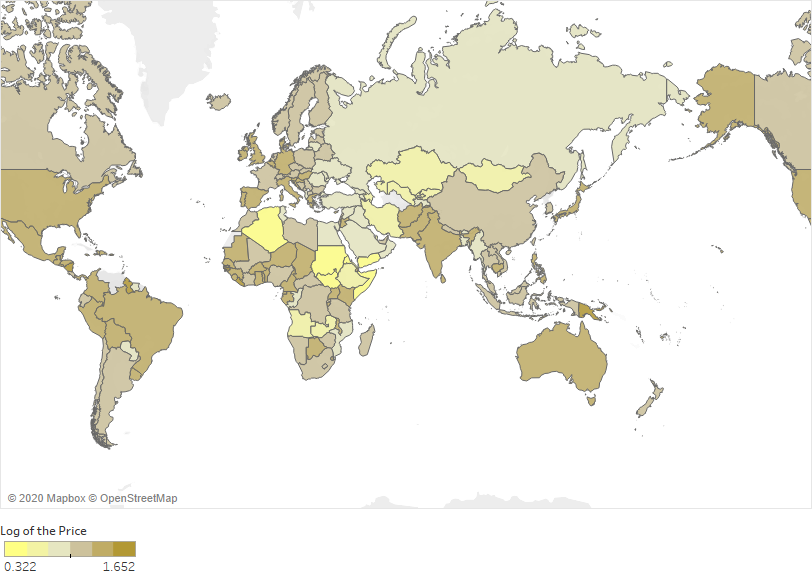
\includegraphics[width=0.7\textwidth]{Images/world2020.png}
\caption{The more expensive electricity is, the darker the color. }
\end{center}
\end{figure}
\bigskip

Some countries are not colored either because their price is too low, as the case is for Kuwait, with less than one cent per kWh, or because too high, as for Solomon Islands and Venezuela. This latter country in recent years has been suffering for exceptional inflation: the take-home message, however, is that the political and macro-economical frameworks are extremely important for the final price of this good.\\

Apart from South America, also in Africa some results are quite interesting: looking at the pale color of countries like South Sudan or Somalia, which are among the poorest in the world, the reader may think that to wealthier country consistently should correspond higher electricity price, given that there is no sky-high inflation. If however, for instance, bordering countries as Algeria and Niger countries are considered, this simple hypothesis does not work: the former has an electricity price of 2.1 dollar cents per kWh and a GDP per capita of 4,114.72 dollars. In the latter, instead, electricity price corresponds to 21.3 dollar cents per kWh (10 times with respect to Algeria) but the GDP is merely 413.98 dollars (almost one tenth with respect to Algeria). Since inflation is not really a problem in Niger, this is a hint that the link between economic development and electricity price is not that elementary. The particular problem with Niger is its extremely low electrification rate: only one in seven Nigeriens have access to modern electricity services, and just four percent of rural residents have access through the national utility. The country's total energy consumption per capita is 44 kWh of electricity. It is the second lowest energy consumption per capita in West Africa, behind Guinea Bissau, and the ninth lowest in the world. 

\section{Access to Electricity}

While the whole share of Algeria inhabitants has access to the grid, this is not the case for Niger, where only part of the relatively wealthier urban population does. This explains why the price is not related with the gross domestic product per capita: since only the wealthy population can afford to have access to the grid, the prices can be kept higher. In this case a loop is entered, since prices are also high because network costs are shared among few people, and network costs are the most important component in the final electricity price paid by households. In \textit{Figure 1.2} it is showed how electricity price (in dollar cents per kWh) is related to population share having grid access, for countries with no universal electricity service.

\bigskip
\begin{figure}[H]
\begin{center}
\captionsetup{justification=centering}
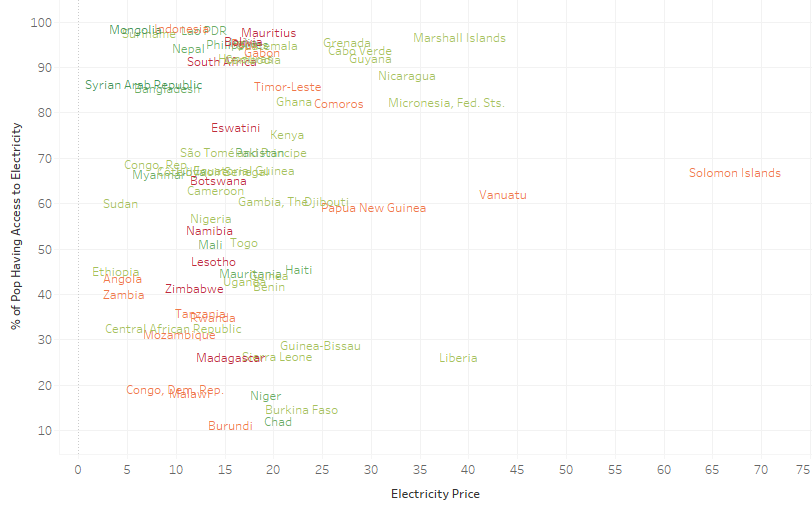
\includegraphics[width=0.85\textwidth]{Images/accessNAMES.png}
\caption{The more southern the country, the redder the color. }
\end{center}
\end{figure}
\bigskip

Although the countries providing little electricity access to their population also have low gross domestic product, prices are not that low with respect to wealthier and more electricity-intensive countries. In \textit{Figure 1.3} it is represented how countries with little grid access are concentrated in Africa: in recent years, Asian countries (especially India) have made important steps forward in this sense.

\bigskip
\begin{figure}[H]
\begin{center}
\captionsetup{justification=centering}
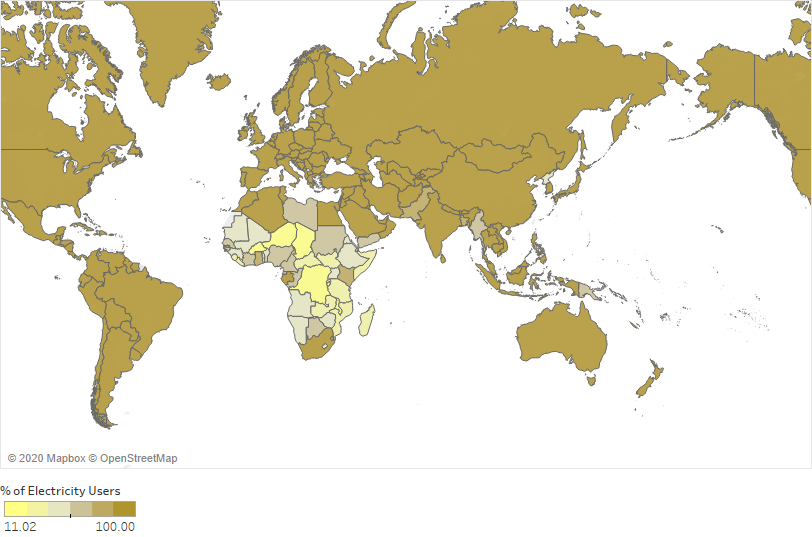
\includegraphics[width=0.7\textwidth]{Images/access.png}
\caption{Share of population having grid access. }
\end{center}
\end{figure}
\bigskip

\section{Production}

Access to electricity is linked to production and consumption patterns inside a country. Electricity is not freely available in nature, so it must be ``produced" (that is, transforming other forms of energy to electricity). Apart from a slight decrease during the 2008 crisis years, electricity production has been increasing constantly in recent years, with China having overcome United States as the main producer.\\

\textit{Table 1} illustrates which are the main electricity generators, with most recent data available. It is interesting to notice the leap of China which was able to increase its generation by five times of the amount it was producing in 2000, with an average increase of 5 percent per year. The United States also increased their production, but not at the pace of China. India was only the $7_{th}$ biggest producer in 2000, and also was able to climb the rankings quite fast in order to allow for its economy to grow. Japan, instead, saw its production decrease in the same time period.

\bigskip
\begin{table}[H]
\begin{center}
\begin{tabular}{|c|c|c|}
\hline
Country & Production (2000) & Production (2019)\\
\hline
China & 1,356 & 7,482\\
United States & 4,053 & 4,385\\
India & 570 & 1,614\\
Russia & 878 & 1,122\\
Japan & 1,068 & 1,013\\
Canada & 606 & 649\\
\hline
\end{tabular}
\caption{Major Electricity Producers (in KwH), Enerdata.}
\end{center}
\end{table}

If the focus shifts to European countries, Germany and France turn out being the two major producers in the continent, followed by the United Kingdom. European situation is illustrated in \textit{Figure 1.4}.

\bigskip
\begin{figure}[H]
\begin{center}
\captionsetup{justification=centering}
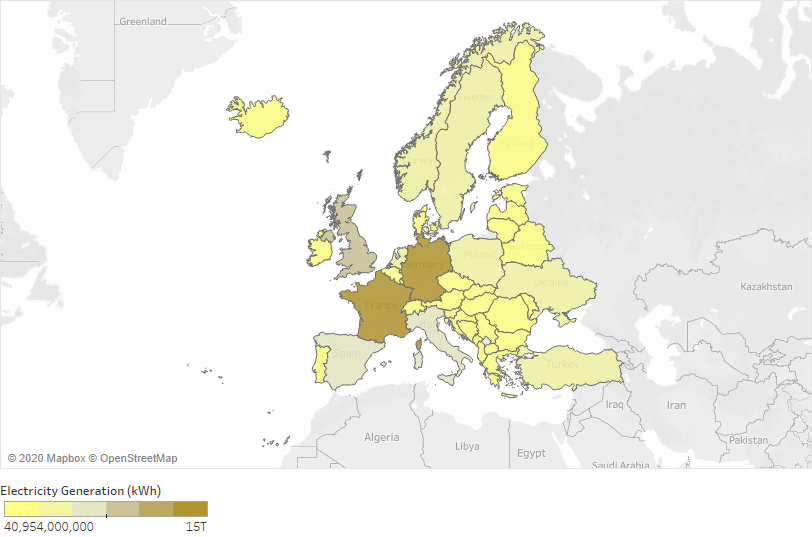
\includegraphics[width=0.8\textwidth]{Images/prod.png}
\caption{European countries and corresponding electricity generation capacity. }
\end{center}
\end{figure}
\bigskip

\section{Distribution}

Of course producing electricity shall be a problem for certain countries, which lack the necessary resources. But an even more significant issue is often the absence of the necessary infrastructure to distribute this good. For poor regions in particular, electricity distribution losses represent  a big concern that hinder their economic development. \textit{Table 1.2} shows which are the countries that have the least efficient electricity distribution infrastructure.

\bigskip
\begin{table}[H]
\begin{center}
\begin{tabular}{|c|c|}
\hline
Country & Losses (\%)\\
\hline
Togo & 71\\
Libya & 69.7\\
Haiti & 60.1\\
Iraq & 50.6\\
Congo, Rep. & 44.5\\
Niger & 41.8\\
\hline
\end{tabular}
\caption{Distribution Losses (\% of output), World Bank data.}
\end{center}
\end{table}

Sadly, most of the distribution losses are associated with very poor countries, in which the access to electricity is limited. 

\section{Consumption}

Since the major costs associated with electricity are actually related to transportation, most of the electricity produced in one country actually remains inside that country until it is consumed. This explains why the major electricity producers are also the major electricity consumers. However, there are still marginal differences among these rankings. \textit{Table 1.3} shows which are the principal electricity consumers in the world.

\bigskip
\begin{table}[H]
\begin{center}
\begin{tabular}{|c|c|c|}
\hline
Country & Consumption (2000) & Consumption (2019)\\
\hline
China & 1,138 & 6,510\\
United States & 3,590 & 3,865\\
India & 376 & 1,230\\
Russia & 693 & 922\\
Japan & 986 & 918\\
South Korea & 263 & 553\\
\hline
\end{tabular}
\caption{Major Electricity Producers (in KwH), Enerdata.}
\end{center}
\end{table}

Also in this case, information regarding Asian countries turns out being the most compelling. China, India and South Korea have experienced a major boost in their electricity consumption while Japan decreased its value in the last 20 years. China is the country which consumes (and produces) the largest share of electricity because it is also the most populated. Data regarding consumption patterns per capita is reported in \textit{Table 1.4}.

\bigskip
\begin{table}[H]
\begin{center}
\begin{tabular}{|c|c|c|}
\hline
Country & kWh consumption per Capita\\
\hline
Iceland & 53,832\\
Norway & 23,000\\
Bahrain & 19,597\\
Kuwait & 15,591\\
Canada & 15,588\\
Finland & 15,520\\
\hline
\end{tabular}
\caption{Countries with highest consumption per capita values, World Bank data.}
\end{center}
\end{table}
\bigskip

There are certain countries that are particularly ill-suited for the existence of individuals, and a large amount of energy has to be consumed in order to improve the well-being o. It is the case of Bahrain or Kuwait where massive amounts of energy are needed to cool buildings. Or, conversely, it is the case of Iceland and Norway, where temperatures are very low and during winter months sunlight is available only for few hours. \textit{Figure 1.5} displays how European countries with highest consumption per capita are located in the North, where temperatures are lowest.

\bigskip
\begin{figure}[H]
\begin{center}
\captionsetup{justification=centering}
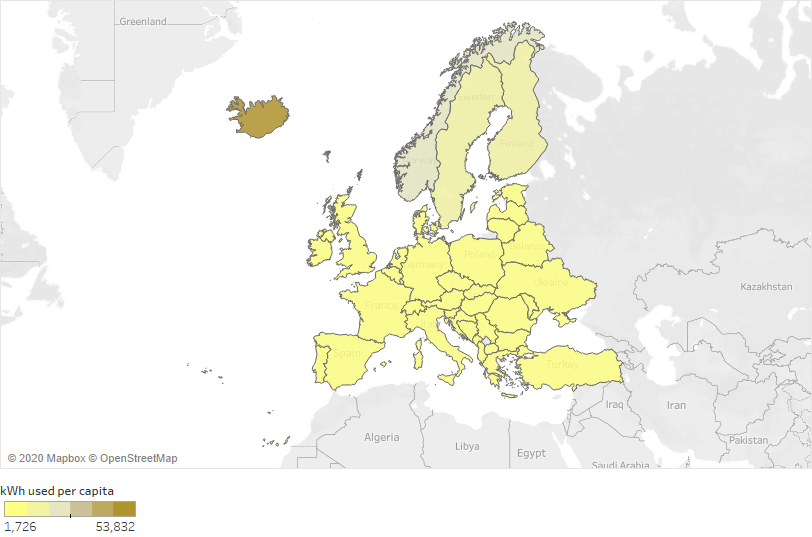
\includegraphics[width=0.75\textwidth]{Images/cons.png}
\caption{European countries and corresponding consumption per capita values, World Bank data. }
\end{center}
\end{figure}
\bigskip

\section{European Union Electricity Market}

Electricity is not an easily tradable product, as it needs hundreds of  legal rules and technical standards to be agreed upon before it can become freely marketable. Electric power is, after all, nothing more than a flow of electrons inside metallic wires of a massive, interconnected network. That is the reason why, for decades, electricity was deemed to be an "anti-market" product, best suited to non-competitive markets like natural monopolies. \cite{glachant2014eu} Furthermore, the particular characteristics of electricity, its non-storability and the necessary constant balance between demand and supply, supported the State intervention. This monopoly predisposition resulted in efficiencies, where State subsidies have been the rule to maintain a stable industry. \cite{domanico2007concentration} Nevertheless, there is one region in the world that has tried to overcome these "anti-market" barriers to create an extremely vast electricity market. That region is identifiable as the European Union. \\

The European Union is a unique case of a large extended market in which member countries can exchange goods.  Liberalization of the economic markets and convergence are two of the main objectives in the Union. In particular, European electricity market liberalization represents the world's most large-scale cross-jurisdiction reform of the electricity sector involving integration of national markets. Reaching such an outcome took several years of time, and there are specific reasons why this process took so long:

\begin{itemize}

\item The objective of this project is to open up national monopolies’ market spaces to foreigners, which of course is a radical
project that inevitably leaves some parties unsatisfied.  One of the risks of market concentration is that big incumbents try to build
barriers in order to maintain their position and to foreclose the entrance of more efficient market actors. \cite{ringel2003liberalising}

\item In the last 25 years there has been no wave of disruptive technological innovation to challenge the incumbent energy
giants.

\item The national arrangements that had been developed between industry players and public authorities could not be easily merged at the EU level into a common scheme.
\end{itemize}

Creating a market that is actually free, however, is not an easy matter, and that's why there are still wide differences in the amounts households from different member countries pay for electricity. Although the pace of the liberalization is steady, the integrated European electricity market is yet to be achieved. \\

\subsection{Taxation}

Taxes account for a sizable share of the final prices consumers pay for energy around the EU and can have a strong impact on consumption patterns, the type of energy consumed and their use. There is disagreement among European countries for how much households should pay in their bills, and the consequence is wide differences in tax rates. Belgium, Ireland, Germany and Denmark are the member states where electricity is the most expensive. However, these four countries present different tax rates: Belgium and Ireland citizens pay a high price because electricity is actually expensive excluding taxes and levies while Germany and especially Denmark pay such a high price precisely because of taxes and levies. This behavior is well represented with \textit{Figure 1.6}, where household electricity prices are plot both including and excluding taxes and levies. Prices are lowest in Bulgaria and Hungary, whose inhabitants pay one third of the amounts Danish citizens pay in their bills. 

\bigskip
\begin{figure}[H]
\begin{center}
\captionsetup{justification=centering}
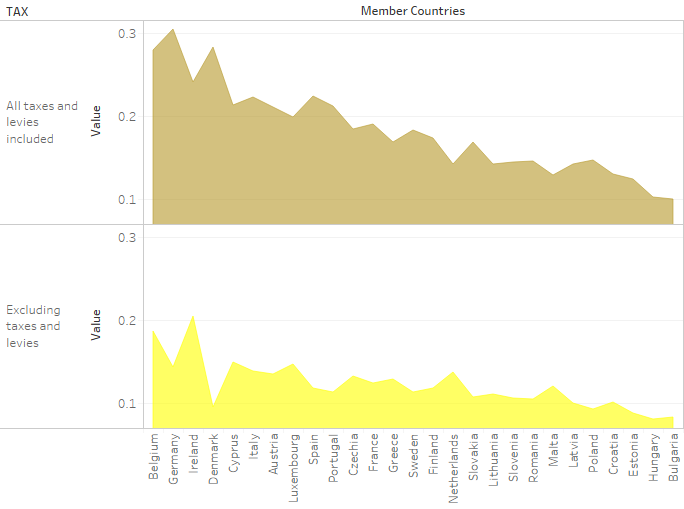
\includegraphics[width=0.7\textwidth]{Images/Taxes.png}
\caption{2019 (second semester) data, electricity prices. }
\end{center}
\end{figure}
\bigskip

The average final price paid by European households is 21.7 cents per KwH including taxes and 12.8 cents per KwH excluding taxes, which make up an average of around 6 cents of taxes per KwH. Over time, also taxes tend to change: in the second semester of 2007 the price paid by European households fell with respect to the first semester by 3 cents, while the electricity price itself decreased only by one cent. This means that most of the drop was due to a decrease in taxes. \textit{Figure 1.7} shows how electricity prices for European citizens changed over time, on average.

\bigskip
\begin{figure}[H]
\begin{center}
\captionsetup{justification=centering}
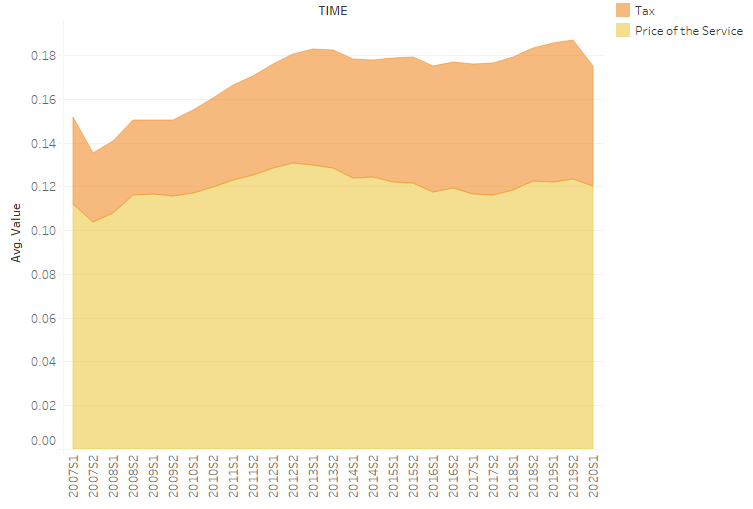
\includegraphics[width=0.7\textwidth]{Images/TaxesTime.png}
\caption{2019 (second semester) data, electricity prices. }
\end{center}
\end{figure}
\bigskip

\subsection{Inflation}

As all other commodities, the price of electricity tends to increase over time at a similar pace with respect to inflation. The average increase in prices in a given country is an obvious cause for electricity price surge. In the European Union the levels of inflation are over time converging, as it should be for such a tied market, and the pace of such convergence became even more steady after the global financial crisis. \cite{brovz2018dynamics} The body which is charge for controlling the inflation level in the Euro area is the European Central Bank, and the primary objective of its monetary policy is to maintain price stability. The ECB aims at inflation rates of below, but close to, 2\% over the medium term. The ECB failed to keep inflation under this level for the first years of the 21th century, before the 2008 financial crisis, but after this the inflation level dropped and never got back to such high levels. Such inflation target was highly debated in recent times, especially after the Federal Reserve has relaxed the same 2\% target.\\

As it is possible to discern from \textit{Figure 1.8}, the inflation level and the electricity price tend to show a similar trend. The average level of prices in 2015 is used as a benchmark and is denoted by a 100 in the plot. Interestingly, however, the electricity price has had its peak in 2012, while inflation continued being positive until now. 

\bigskip
\begin{figure}[H]
\begin{center}
\captionsetup{justification=centering}
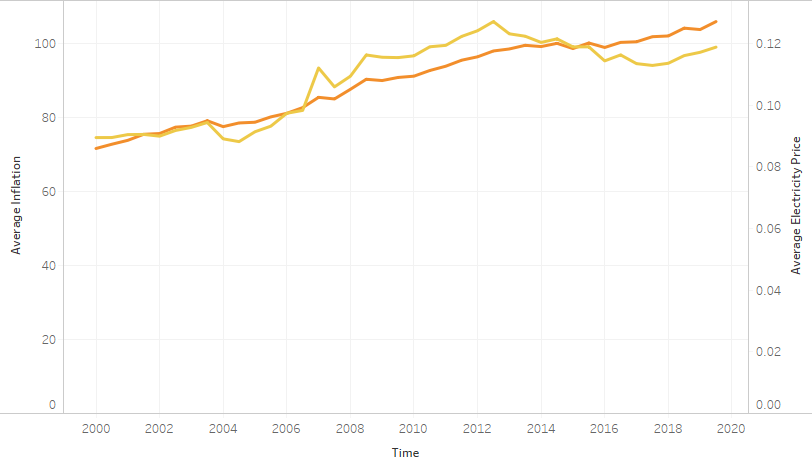
\includegraphics[width=0.8\textwidth]{Images/inf.png}
\caption{Price of electricity and inflation level in the European Union . }
\end{center}
\end{figure}
\bigskip

The behavior of inflation depends both on structural and on short-term factors. The inflation rate over long periods is determined by the extent to which the rate of money growth (which is controlled by the ECB or by national central banks in non-euro countries) exceeds the growth rate of real output. Short-run fluctuations are instead due to demand shocks, e.g. sizable increases in government spending, and supply shocks, e.g. sharp rises in the oil price. \cite{ball1993causes}

\subsection{Market Concentration}

The directive 2003/54/EC requires that all non-household customers can freely choose their electricity supplier by 1 July 2004, with following full market opening including all household customers within three years. Most of the European Union electricity market is now at least formally, open to competition; this was not the case a few decades ago. However, most national electricity markets are still controlled by relatively few companies and small consumers seem quite resistant to switching supplier. \cite{jamasb2005electricity} \\

The European Union is fighting monopolies in the electricity sector for the simple reason that the market price is supposed to be higher with respect to a situation of competition. In the 1990s the United Kingdom was the front-runner of electricity reforms, while France has often been regarded as a country averse to moving away from public monopoly. \cite{fiorio2009reform} In \textit{Figure 1.9} European countries are colored according to their level of market concentration. It is possible to notice how, most notably, the market concentration levels are quite heterogeneous among countries, with France, Estonia and Croatia experiencing very different levels with respect to United Kingdom, Poland and Spain. 

\bigskip
\begin{figure}[H]
\begin{center}
\captionsetup{justification=centering}
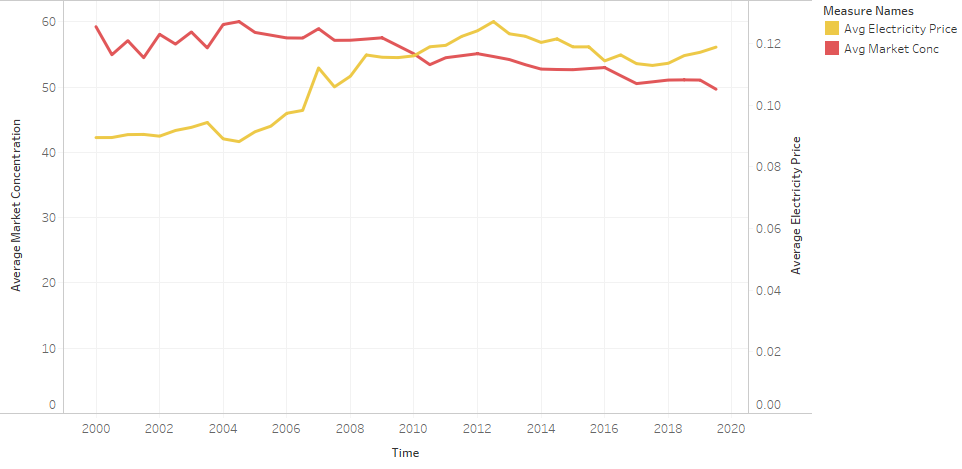
\includegraphics[width=0.6\textwidth]{Images/conc.png}
\caption{Market Share of Largest Producers for European countries, 2018 data. }
\end{center}
\end{figure}
\bigskip

In any case, \textit{Figure 1.9} also demonstrates how, although the liberalization process has led to the disintegration of national monopolies, it did not lead to a disruptive fall in concentration within the sector. With an average value of the biggest  supplier market share of 50\% the European situation is quite far from the internal market and open competition. Different national and regional markets with the presence of incumbents as main actors still persist in each electricity market. Despite liberalization, the level of concentration is hence quite high.  In \textit{Figure 1.10}, the focus shifts to the biggest European markets over the last 20 years: Germany, Spain, France and Italy. It is interesting to notice how they all experienced a slight decrease in market concentration, but with France starting from a concentration value that stands out with respect to the others, with the most important supplier having a market share of 90\%.

\bigskip
\begin{figure}[H]
\begin{center}
\captionsetup{justification=centering}
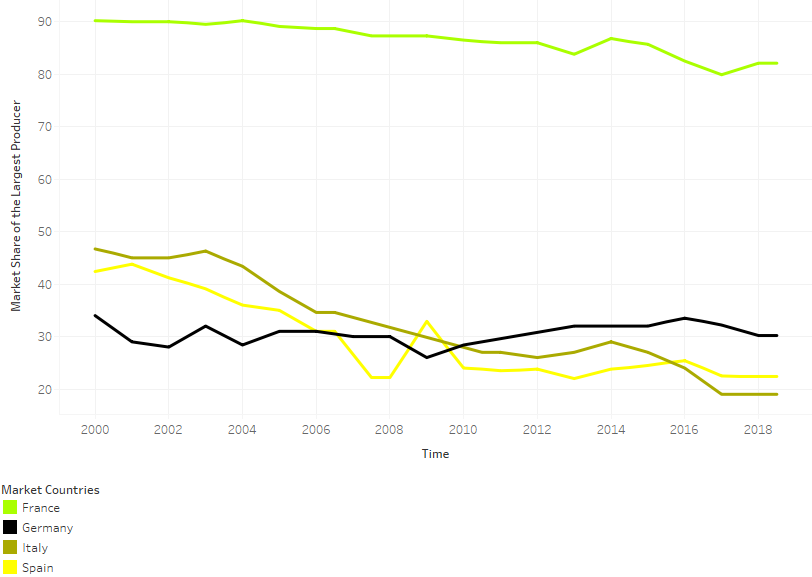
\includegraphics[width=0.6\textwidth]{Images/conc-mc.png}
\caption{Largest supplier market share for Germany, Spain, France and Italy over time. }
\end{center}
\end{figure}
\bigskip

One final note of caution: in this section the market share of the biggest supplier in the market was used as a proxy for market concentration. The lower the share, the more the market is liberalized. However, looking at the largest supplier is a bit limiting and it is used because it is the only information Eurostat discloses about this matter. A market in which only two suppliers share the whole market is completely different from one in which the biggest supplier controls half of the market and the rest of it is controlled by very little providers. Yet, the largest supplier market share variable value would be the same.

\subsection{Gross Domestic Product}

The wealth and the productive capacity of a country are closely related to the consumption patterns of its citizens. Economic development stimulates greater demand for electricity in the long-run: the gross domestic product has an effect primarily on the quantity of electricity consumed. \cite{jamil2010relationship} Whether there is an effect not only on the quantity used but also on the price of the good is a more debated topic: \cite{lean2010multivariate} employs annual data for Malaysia from 1970 to 2008 to examine this causal relationship but found that there is no causal relationship between prices and economic growth. \textit{Figure 11} displays the differences in GDP per capita for European countries. \footnote{World Bank data}

\bigskip
\begin{figure}[H]
\begin{center}
\captionsetup{justification=centering}
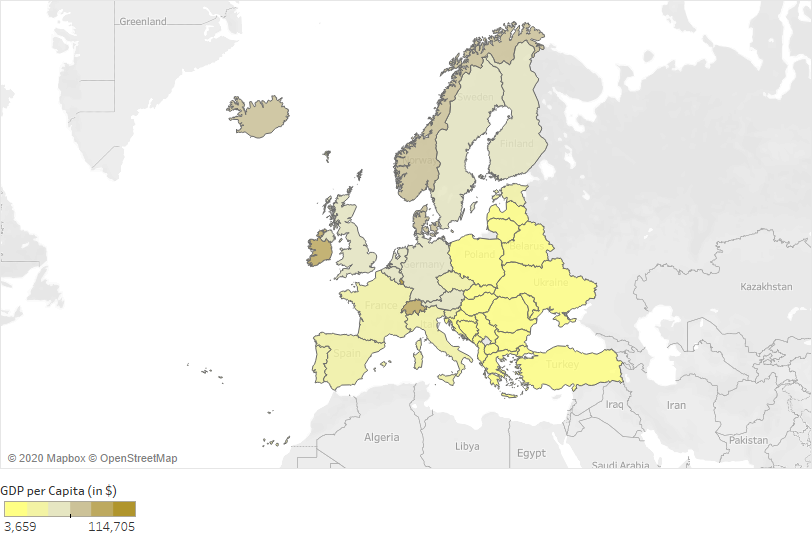
\includegraphics[width=0.6\textwidth]{Images/gdp.png}
\caption{Gross Domestic Product per capita for European countries (in Dollars). }
\end{center}
\end{figure}
\bigskip

Belgium, Ireland, Germany and Denmark are the European member countries for which electricity is the most expensive, and these four areas also show high GDP value. In the last 20 years Gross Domestic Product tended to increase for European countries, even if the economic crisis incurred in the end of the first decade slowed down the growth process. Also the electricity price has tended to increase, although at different paces and more irregularly with respect to the Gross Domestic Product.\\

\textit{Figure 1,12} shows the behavior of real GDP per capita and electricity price (taxes excluded) for France and Germany, the two major economies in the European Union.  In this case inflation has been taken into account and in fact the absolute GDP values are not comparable with \textit{Figure 1.11}. Electricity is cheaper in France with respect to Germany by quite a significant amount, and Gross Domestic Product is also lower. For both countries there has been an increase in the values of the two variables, although with considerable less regularity when it comes to electricity price.

\bigskip
\begin{figure}[H]
\begin{center}
\captionsetup{justification=centering}
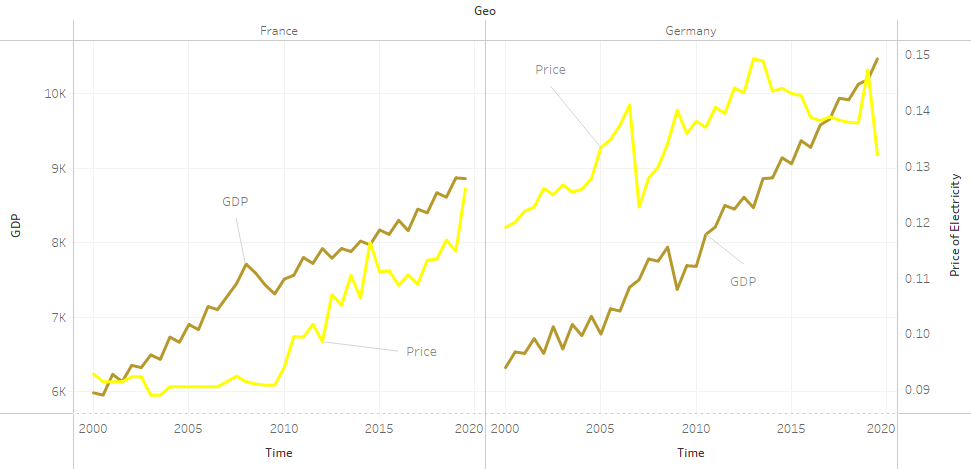
\includegraphics[width=0.8\textwidth]{Images/pri-gdp.png}
\caption{GDP per capita and Electricity Price over time for France and Germany. }
\end{center}
\end{figure}
\bigskip

\subsection*{Emission Intensity}

Depending on how it is produced, electricity can be associated with environmental degradation. A debated question in recent times is whether cleaner energy results in higher prices or rather the opposite. The \textit{Emissions Intensity} indicator is calculated as the ratio between energy-related GHG emissions and gross inland consumption of energy. It expresses how many tonnes CO2 equivalents of energy-related GHGs are being emitted in a certain economy per unit of energy that is being consumed.\\

All European countries successfully managed to decrease their emission intensity in the last 20 years, but with wide differences. Eastern countries which base their economy on energy production and distribution such as Ukraine and Georgia saw their emission intensity levels drop by one tenth in one year. Such result is mostly due to the very low levels of efficiency these countries were experiencing in the beginning of the century. In \textit{Table 4} emission intensity for most virtuous countries is summarized: the relative level in the table is benchmarked over the emission intensity level the country experienced in 2000 (i.e. level in 2000 = 100).

\bigskip
\begin{table}[H]
\begin{center}
\begin{tabular}{|c|c|}
\hline
Country & Emission Intensity \\
\hline
Ukraine & 90.9\\
Malta & 90.9\\
Georgia & 90.9\\
Kosovo & 91.3\\
Moldova & 91.3\\
\hline
\end{tabular}
\caption{Countries which reduced their emission intensity the most in the last 20 years.}
\end{center}
\end{table}
\bigskip

With \textit{Table 1.6}, instead, a summary is provided the countries which experienced the smallest drop in emission intensity in the last 20 years. It may be not that easy to match economic development with climate action, and progress in one field can hinder progress in the other.

\bigskip
\begin{table}[H]
\begin{center}
\begin{tabular}{|c|c|}
\hline
\rowcolor{lightgray}Country & Emission Intensity \\
\hline
Bulgaria & 97\\
Lithuania & 95.6\\
Luxembourg & 95.3\\
Cyprus & 95.2\\
Estonia & 95\\
\hline
\end{tabular}
\caption{Countries which reduced their emission intensity the most in the last 20 years.}
\end{center}
\end{table}
\bigskip

Eurostat does not provide absolute values for the Emission Intensity indicator, but the World Bank provides data for $CO_{2}$ emissions per capita. \textit{Figure 1.13} helps to visualize the countries which are the most and least $CO_{2}$ intensive. One interesting area of focus for further discussion is the Baltic. To demonstrate how political decisions can result in building two radically different economies also for countries which are neighboring and similar, it is interesting to notice how Lithuania is one of the least polluting country in Europe and Estonia is instead the one that is polluting the most.

\bigskip
\begin{figure}[H]
\begin{center}
\captionsetup{justification=centering}
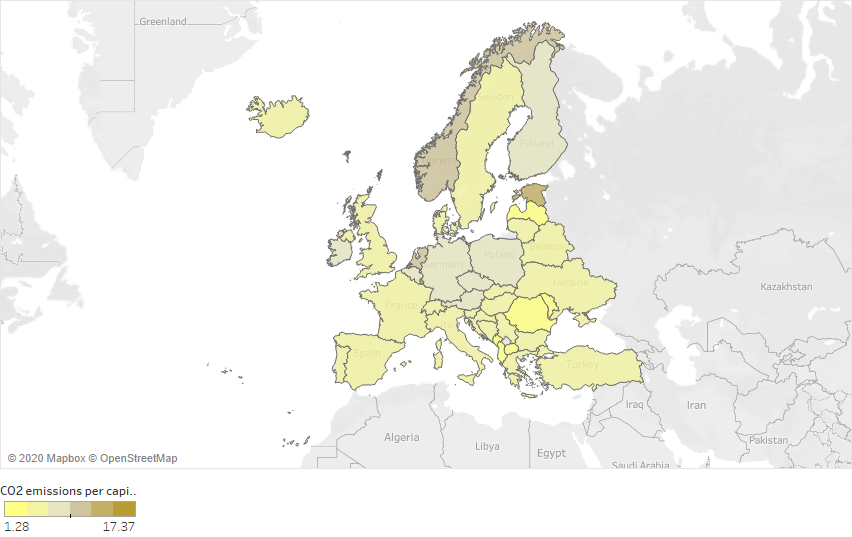
\includegraphics[width=0.7\textwidth]{Images/intensiti.png}
\caption{CO2 emissions (metric tons per capita). }
\end{center}
\end{figure}
\bigskip

\subsection*{Energy Mix}

The importance of energy on greenhouse gases emissions is reflected by the fact that 65\% of emissions in the World are currently due to the use and production of energy. This percentage rises up to 80\% in the European Union.\cite{marrero2010greenhouse} Energy production techniques and consequent polluting emissions vary greatly from one country or region to the other and can change significantly depending on the period. The term \textit{energy mix} refers to the combination of the various primary energy sources used to meet energy needs in a given geographic region. Variables at stake for the final choice of the energy mix include:

\begin{itemize}

\item The availability of resources domestically or the possibility of importing them;
\item The demand of energy which needs to be met;
\item Policy choices determined by political, economic, environmental and geopolitical factors.

\end{itemize}

Low income, developing countries tend to rely heavily on biomass energy and coal. \cite{international2009energy} As countries become wealthier, new technologies enter the market, and they substitute towards higher quality energy sources. \cite{csereklyei2016energy}

\subsubsection*{Coal}

Although the EU electricity system has innovated and become greener, it has also maintained its oldest and most polluting component: coal. As mentioned above, it is usually under-developed countries that rely heavily on coal. However, political decisions are also key in this sense. Poland has seen its economy grow steadily in recent years, but still relies heavily on coal for electricity production. European countries which count on coal the most are listed in \textit{Table 1.7}.

\bigskip
\begin{table}[H]
\begin{center}
\begin{tabular}{|c|c|c|}
\hline
\rowcolor{lightgray} \multicolumn{3}{|c|}{Electricity Prod. from Coal (\% of total)}\\
\hline
Country & 2015 & 2000 \\
\hline
Kosovo & 97.5 & 97.6\\
Poland & 80.91 & 96.3 \\
Serbia & 72.4 & 62.8 \\
Bosnia & 63.4 & 50.7\\
North Macedonia & 58.4 & 76.5\\
\hline
\end{tabular}
\caption{Countries which rely on coal sources for electricity generation the most.}
\end{center}
\end{table}
\bigskip

The trend in reducing the impact of coal in the energy mix has been set in all corners of Europe, and now the focus is on the timing. Even Germany, a country which is very careful on environmental matters, in 2015 still relied on coal for 44\% of its energy production. The share of fossil fuel in the EU electricity generation mix stands at 25 percent, having declined by only 5 percentage points between 2000 and 2015. This is a problem, since as \cite{tagliapietra2017beyond} points out, to generate the same amount of electricity, a coal-fired power plant emits 40 percent more CO2 than a gas-fired power plant and 20 percent more than an oil-fired power plant. \textit{Figure 1.14} displays where major EU countries are in the path towards decarbonization.

\bigskip
\begin{figure}[H]
\begin{center}
\captionsetup{justification=centering}
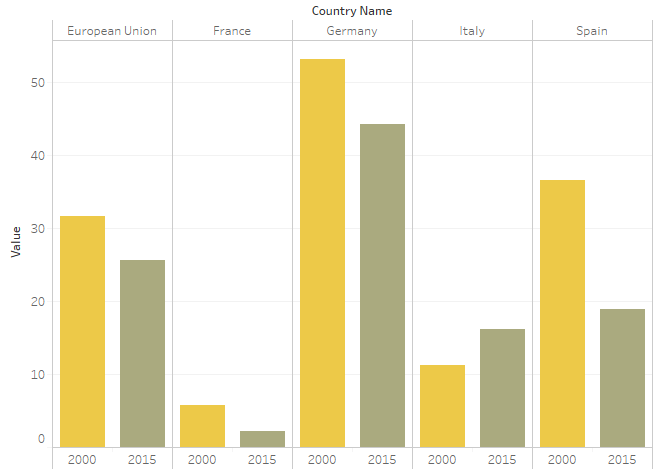
\includegraphics[width=0.5\textwidth]{Images/coal.png}
\caption{Electricity Production from Coal (\% of total). }
\end{center}
\end{figure}
\bigskip

\subsubsection*{Oil}

One traditional way of producing electricity is by fuel combustion: the raw material, oil, sits in deep underground reservoirs. Since the ultimate amount of oil is finite - and cannot be replenished once it is extracted and burned - it is not a renewable resource. Burning oil to generate electricity produces significant air pollutants, and this may also explain why this energy source is going out of fashion: in the 70s oil combustion was one of the main techniques for electricity generation, accounting for about one fifth of the total. In following years, however, this share started to shrink constantly: in 2015 only less than 4\% of electricity is generated by fuel combustion. \textit{Figure 1.15} shows the trend in electricity generation from fuel combustion.

\bigskip
\begin{figure}[H]
\begin{center}
\captionsetup{justification=centering}
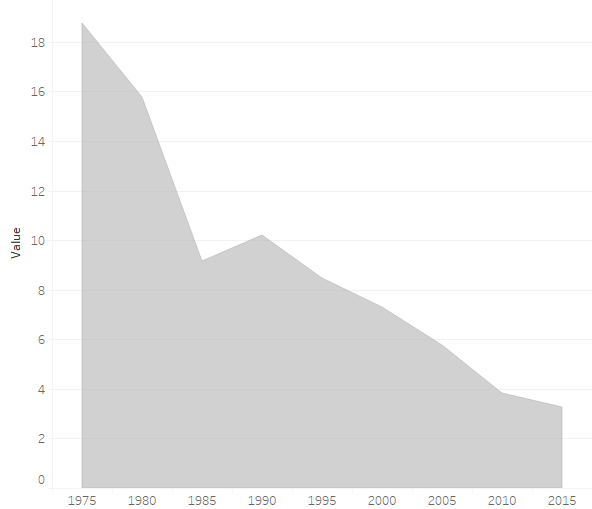
\includegraphics[width=0.5\textwidth]{Images/oil.png}
\caption{Electricity Production from Oil (\% of total). }
\end{center}
\end{figure}
\bigskip
 
Since oil can be used for producing electricity, one could easily infer that the price of the former could have an effect on the price of the latter. Oil price has showed significant fluctuations in the last 20 years. From 1999 until mid 2008 the price of oil rose significant thanks to the rising oil demand in Asian countries. The 2007-2008 financial crisis corresponded to a drop in the price of crude oil, followed by a fast recovery in the following years. The world price of oil was above 125 US dollars per barrel in 2012, and remained above \$100 until September 2014, after which it entered a sharp downward spiral, falling below \$30 by January 2016. What happened is the so-called \textit{oil glut}, a serious surplus of crude oil that started in 2014 and accelerated in the next two years, with multiple causes. These include general oversupply as United States and Canadian oil production (obtained by fracking) reached critical volumes, geopolitical rivalries among oil-producing countries, falling demand across markets due to the slow down of the Chinese economy, and possible restraint of long-term demand due to environmental concerns. \textit{Figure 1.16} represents graphically what happened in the last 20 years, with all the up and downs the price of oil experienced.

\bigskip
\begin{figure}[H]
\begin{center}
\captionsetup{justification=centering}
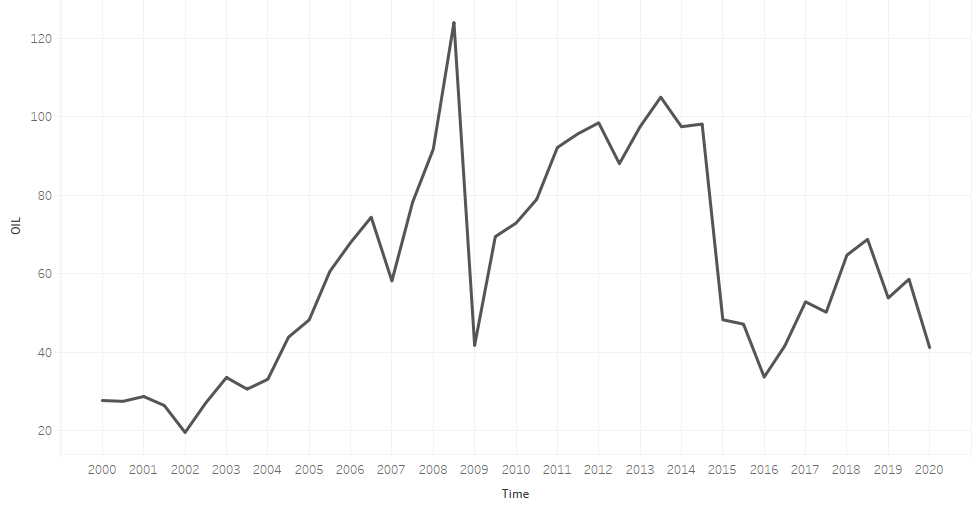
\includegraphics[width=0.6\textwidth]{Images/oilbeh.png}
\caption{Electricity Production from Oil (\% of total). }
\end{center}
\end{figure}
\bigskip

\subsubsection*{Nuclear Power}

Electricity can also be produced by a process which makes use of nuclear reactions. This type of energy has one of the lowest levels of fatalities per unit of energy generated compared to other energy sources, given that electricity generation by coal and oil combustion result in air pollution. \cite{markandya2007electricity} However, nuclear power is going out of fashion mostly because of Chernobyl and Fukushima disasters, which questioned its use in Europe. Germany was one of the most radical governments to abandon its nuclear energy program, having the greatest number of permanently closed nuclear plants among the 27 European Union member countries. In fact, it plans to shut down all remaining nuclear reactors by 2022. Having taken opposite political decisions, France still relies heavily on nuclear power generation. It has the second highest number of operable nuclear reactors worldwide and it is supposed to build an additional nuclear reactor. Leaving out France, most of the other European countries are going in the direction of a reduction in the share of energy produced by nuclear reaction. Only Slovakia is greatly investing in broadening its nuclear energy program, looking to add two further reactors to the four already in use. \textit{Table 1.8} summarizes the trend in nuclear energy production: the share of energy produced by reactors as percentage of the total in 2000 and 2015 is displayed.

\bigskip
\begin{table}[H]
\begin{center}
\begin{tabular}{|c|c|c|}
\hline
\rowcolor{lightgray} \multicolumn{3}{|c|}{Nuclear Energy (\% of total)}\\
\hline
Country & 2015 & 2000 \\
\hline
France & 77.6 & 77.6 \\
Slovakia & 56.9 & 53.6 \\
Hungary & 52.2 & 40.3 \\
Slovenia & 38.1 & 35 \\
Belgium & 37.5 & 58.1\\
\hline
\end{tabular}
\caption{Countries which rely on nuclear reactors for electricity generation the most.}
\end{center}
\end{table}
\bigskip

\subsubsection*{Renewable Sources}

The use of renewable energy for producing electricity has several potential benefits, including a reduction in greenhouse gas emission and a reduced dependency on fossil fuel markets (in particular, oil and gas). Additionally, it is considered safer with respect to nuclear production, due to the disasters experienced in the last 40 years. The increase in the share of electricity produced through renewable sources has been steady in the last 20 years, going from a share of 9.6\% of the total in 2004 to 18.9\% in 2004. While the EU as a whole is on course to meet its 2020 targets, some member states will need to make additional efforts to meet their obligations.
\textit{Figure 1.17} shows where each country is in the path towards more sustainable energy sources.

\bigskip
\begin{figure}[H]
\begin{center}
\captionsetup{justification=centering}
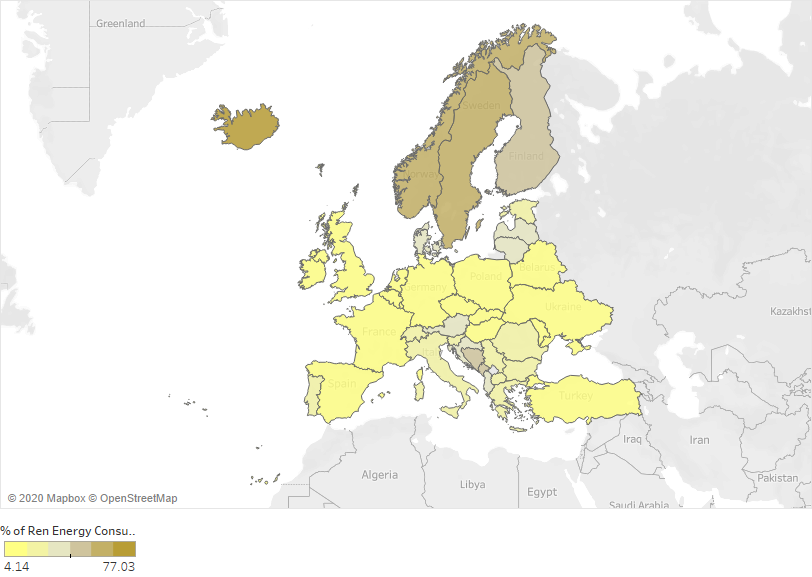
\includegraphics[width=0.7\textwidth]{Images/ren.png}
\caption{Renewable Energy Consumed (\% of total). }
\end{center}
\end{figure}
\bigskip

Northern countries have invested significantly in renewable energy sources and the result is that their achievements in the path towards sustainability are particularly strong. Iceland is particularly strong in geothermal energy while Sweden and Norway make use of their considerable supply of moving water and biomass. In fact, renewable energy sources are a broad categorization including:

\begin{itemize}
\item \textit{Hydro Power}, which is the most relevant renewable energy source. Since water is so dense, even a slow flowing stream can result in a sizable amount of energy.
\item \textit{Geothermal Power}, which is obtained from thermal energy stored in the ground.
\item \textit{Biomass}, which can either be used directly via combustion to produce heat, or indirectly by converting it into biofuel.
\item \textit{Wind Power}, which is preferred in areas where winds are strong and constant, as in the case of high-altitude sites.
\item \textit{Solar Power}, which is having a rapid increase in importance. Italy has the largest proportion of solar electricity in the world (7.7\% in 2015).
\end{itemize}

The fact that in recent times the energy mix has changed so much, moving to cleaner options, has an important effect for the electricity market too. Whether such an effect is going to influence also the price of the good is going is one of the points of focus of the next chapter.

\subsection{Dependency}

European Union member states import a lot of energy from other countries, as Norway and Russia. In total, the dependency rate was equal to 58 \% in 2018, which means that more than half of the EU’s energy needs were met by net imports. The result is that Europe relies heavily on them for its supply and to a certain extent has to conform to others' prices. In \textit{Table 1.9} dependency on imports for European countries is summarized. Malta, which lacks the necessary resources for producing electricity and is not really interested in investing in renewables, represents the example of a country which entirely depends on abroad sources for its electricity capacity. At the moment none on the European Union countries is self-sufficient, although Denmark in the beginning of the century was thanks to the North Sea production of oil and gas.

\bigskip
\begin{table}[H]
\begin{center}
\begin{tabular}{|c|c|c|}
\hline
\rowcolor{lightgray} \multicolumn{3}{|c|}{Electricity Dependence (\%) }\\
\hline
Country & 2010 & 2018 \\
\hline
Austria & 62.8 & 64.3 \\
Belgium & 77.9 & 24.3 \\
Bulgaria & 40.1 & 82.3 \\
Cyprus & 100 & 92.5 \\
Czech Rep & 25.3 & 36.7\\
Germany & 60 & 63.6 \\
Denmark & -16 & 23.7 \\
Estonia & 15.5 & 0.7 \\
Greece & 68.6 & 70.7 \\
Spain & 77.1 &  73.3 \\
Finland & 48.8 & 44.9 \\
France & 48.7 & 46.6 \\
Croatia & 46.7 & 52.7 \\
Hungary &  56.9 & 58.1 \\
Ireland & 87.1 & 67.4 \\
Lithuania & 79 & 74.2 \\
Luxembourg & 97 & 95.1 \\
Latvia & 45.5 & 44.3 \\
Malta & 99 & 97.8 \\
Netherlands & 28.3 & 59.7 \\
Poland & 31.6 & 44.8 \\
Portugal & 75.2 & 75.6 \\
Romania & 21.4 & 24.3 \\
Sweden & 37.8 & 29.2 \\
Slovenia & 49.5 & 51.3 \\
Slovakia & 64.4 & 63.7 \\
\hline
\end{tabular}
\end{center}
\caption{Dependency on electricity imports. }
\end{table}
\bigskip

\chapter{Methodology}

Many authors have tried to measure the effect of market liberalization and green energy investment, starting from \cite{moreno2012electricity}, in which the analysis  is performed on European Union member countries markets'. The authors from \cite{nagayama2009electric} take a broader perspective, looking at more countries but with older data. The cause-effect analysis is carried out in these studies with an econometric approach, without splitting the data in different subsets for training and validating the results, fact that represents one of the main novelties of the method implemented here.\\

The main focus is on predicting how prices for electricity are going to evolve in the future, and not merely on understanding the causal relationship. In this sense, while the European Union is the main market on which the analysis is based, also \textit{World Bank} data is used as a source of information for countries all over the world. This section is structured as follows: first, models are built on top of \textit{Eurostat} data sets, and then to benchmark those findings, the most global patterns are investigated.

\section{Static European Models}
\subsection{Variables}

The variables in consideration for the European market models seek to resemble the factors listed in the introduction. The response variable, electricity price itself, is expressed in \textit{Euros} and involves households who consume between 2 500 and 5 000 kWh. This means that the focus is on a certain category of consumers: families and not industries. For a panel data analysis on non-household consumers please instead refer to \cite{del2019industrial}.  The price used in the models as response variable does not include taxes. Most remarkably, electricity prices information is recorded twice a year, so in the models year variability is accounted. The time range chosen for the analysis is the last 20 years, from 2000 to the first semester of 2020. This makes the data at hand and the consequent results extremely up-to-date. Minor adjustments had to be carried out because of inconsistencies in the way of recording information between years prior to 2007 and years that follow. The electricity price is going to serve as the outcome variable in the later discussion, and referred as \textbf{PRI}, for short.\\

The two main bills households receive contemplate electric power and \textbf{natural gas}, for cooking, heating, lighting and using domestic appliances inside the building. The two goods are strictly related, because electric power can be produced from gas, and because electricity can represent a substitute of gas (e.g.\ for households that use induction cooktops). Data is taken from \textit{Eurostat} and is also in this case bi-annual and measured in \textit{Euros}. Taxes and levies are not considered: the price is the sum of the raw material value and the cost of transportation and distribution. \textit{Figure 2.1} shows the distribution of the gas price, with the median being around 10 - 11 euros per mega joule. In the later model discussion this variables is going to be named \textbf{GAS}, for short.

\bigskip
\begin{figure}[H]
\begin{center}
\captionsetup{justification=centering}
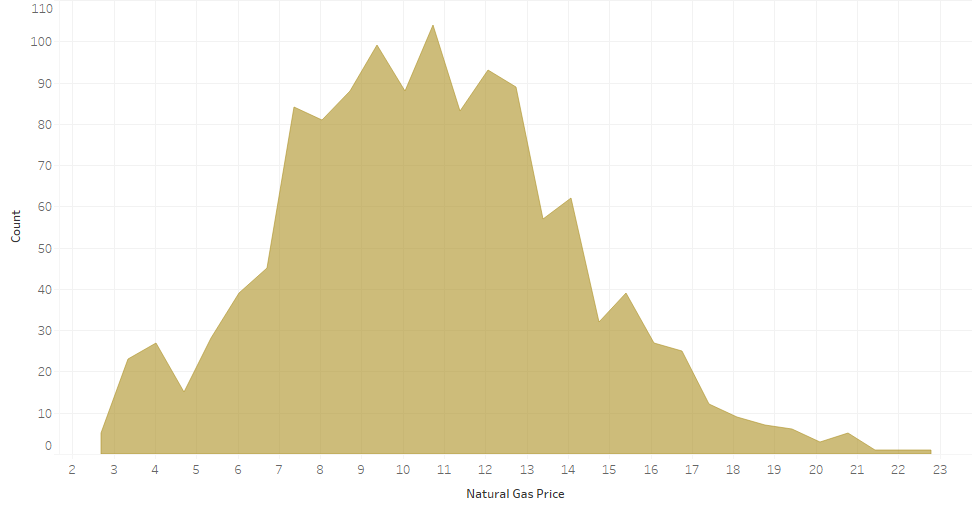
\includegraphics[width=0.7\textwidth]{Images/nGas.png}
\caption{Natural Gas Price Distribution.}
\end{center}
\end{figure}
\bigskip

The idea is to use the price of the resources from which electricity is produced to have an idea of what the price of the good could be. The choice of having the natural gas price as a variable in the data set goes in this sense. It would be reasonable to actually do the same for oil, but \textit{Eurostat} does not disclose any information regard this good price. Options could be either to use the US dollar price per barrel or the pump price for gasoline. The choice falls on the latter, being considered as a good proxy for the price of oil in the country. The data is available from the World Bank, and observations are recorded once every two years. In the later models it is going to be referred as \textbf{OIL}, for short.\\

Electricity, as discussed in the introduction, is not only produced by burning coal, oil or natural gas, but also by using \textbf{renewable resources}. The share of electricity produced using sustainable practices on the total of electricity produced by each single country is also included in the data set, and named as \textbf{REN}, for short. This information is recorded once a year and available from \textit{Eurostat}. However, some years the information is incomplete, specifically those before 2004, so those missing records are topped up with data from \textit{World Bank}. The sets from the two different sources describe the same information, e.g. for data regarding 2004, numbers are almost equivalent: however, just pasting data could be dangerous so normalization of the world bank information is carried out by multiplying each country value for 2000-2003 by a factor that makes records for 2004 match for both sources. \\

\noindent Another variable that takes in consideration the level of sustainability of the electricity produced is the emission \textbf{intensity}. This indicator is used to monitor progress towards United Nations' goal on climate action and on affordable and clean energy and, as anticipated in the introduction, it is calculated as the ratio between energy-related GHG emissions and gross inland consumption of energy. The data on energy emissions are being sourced from the GHG emissions reported to the UNFCCC. Information is normalized with respect to year 2000, which is used as a benchmark. This variable hence expresses how fast that particular economy is in its path towards decarbonization. Data is recorded annually and sourced from \textit{Eurostat}: in the later discussion it is going to be referred as \textbf{EMI}, for short.\\

\noindent It is also important to consider the supply side in this context: how much each country is consuming in terms of energy. \textit{Eurostat} provides information regarding the quantity of oil equivalent (in kilograms), and this data is recorded annually. This indicator measures how much energy every citizen consumes at home excluding energy used for transportation. Since the indicator refers to final energy \textbf{consumption}, only energy used by end consumers is considered. The related consumption of the energy sector itself is excluded. This variable is going to be shortened as \textbf{CON} in the following model discussion.\\

\noindent Many European countries do not really have the capacity to produce enough electricity in order to be self-sufficient. The \textbf{dependency} indicator shows the share of total energy needs of a country met by imports from other countries. It is calculated from energy balances as net imports divided by the gross available energy. The formula for computing the dependence is: $$ \scalebox{2} {$\frac{(imports – exports)}{gross\;available\;energy}$}.$$ A negative value indicates a net exporter: a country that exports more fuels than it consumes. In the context of the data set at hand this happens only for \textit{Norway}. Values higher than 100 generally refer to the build of stocks (increase of fule in stocks), yet might be also a result of statistical discrepancies in raw data. This information is available from \textit{Eurostat} and recorded once a year. This variable is going to be shortened as \textbf{DEP} in the models discussed later.\\

\noindent In the last 20 years the major change in the way electricity is sold is the \textbf{liberalization} forced to member countries by the European Union authorities. The only data regarding the structure of the markets member countries disclosed by \textit{Eurostat} indicates the market share of the largest electricity generator. This information is disclosed annually, and in the following models it is going to appear as \textbf{MAR}, for short. As also discussed in the Introduction, to rely merely on the share of the largest generator may not be enough for having a solid idea of the structure of the market may be sometimes not adequate. The best indicator for market concentration is the HHI (Herfindahl-Hirschman Index) \cite{viscusi2018economics}, and it is computed by adding the square root of the percentage market share of each individual firm in the industry.\\

\noindent The electricity price is also, and maybe most importantly, dependent on how wealthy that single country is. \textit{Eurostat} provides the value of the \textbf{real gross domestic product} per capita, with data being published every quarter of year. ``Real" in this context means deflated, so leaving prices unchanged. This is key: while the gross domestic product tends to increase every year (given that the country is an in inflation regime), the real GDP might be decreasing if, at those prices level, on average the citizens have a lower purchasing power. The reader could wonder why to exclude the average increase in prices from the consideration, although there is a clear correlation between price increase and electricity price: the higher the increase in prices the higher the expected increase in the electricity bill. The answer lies in the fact that the \textbf{inflation} variable \textit{hides} the electricity price change variable itself: the average increase in prices is computed on a basket of goods electricity is part of, so it would be too easy to actually use this variable in the models. The outcome variable exogeneity assumption would not be met. In the following models, the real Gross Domestic Product per capita variable is going to be called \textbf{GDP}, for short.

\subsection{Countries}

\textit{Eurostat} provides information regarding the variables above mentioned for the members of the Union, of course, but also for some neighboring countries, which are included in the study. The idea is to understand whether the membership to the Union does have an effect when trying to predict the final price for electricity. \textit{Figure 19} shows which are the European countries included in the study.

\bigskip
\begin{figure}[H]
\begin{center}
\captionsetup{justification=centering}
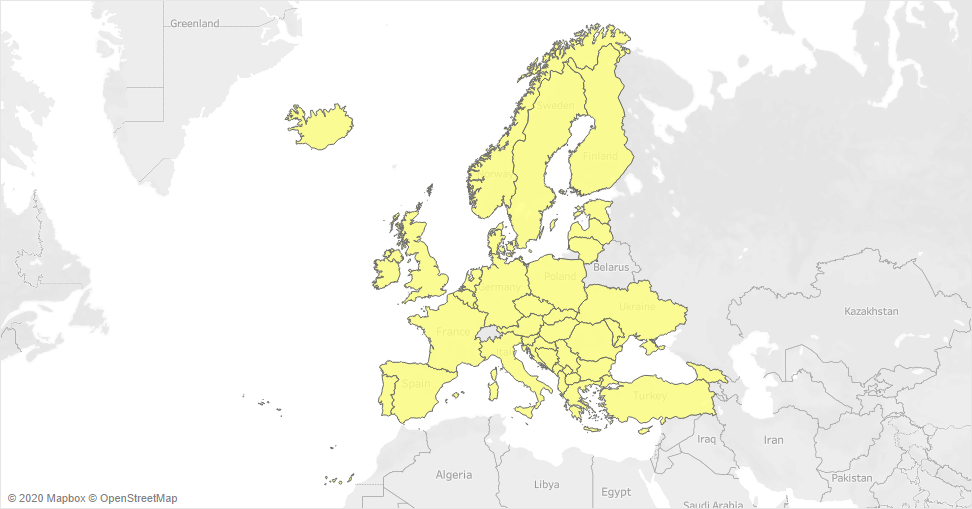
\includegraphics[width=0.8\textwidth]{Images/cantries.png}
\caption{Countries which are included in the study.}
\end{center}
\end{figure}
\bigskip

As discussed in the previous subsection, most information data are not disclosed twice a year but only once: instead of dropping those rows where information data is not available, the mean between the previous and the following semester is computed and inserted in the data set. Other missing data substitution techniques are more sophisticated: for instance, Netherlands does not disclose information regarding electricity market concentration levels. To have an idea of the retail market for this country, an interesting reference is \cite{mulder2019dutch}.  The way out of this found for not discarding Netherlands from the analysis is to substitute those Not Availables with average values from markets with a similar structure, which are Germany, Denmark, Luxembourg and Belgium.

\subsection{Random Effects}

Statistical models always describe variation in observed variables in terms of systematic and unsystematic components. In econometrics, a random-effects model is a statistical model in which some of the parameters (effects) that define systematic components of the model exhibit some form of random variation.\cite{salkind2010encyclopedia} In the context of the problem at hand, which is the electricity price prediction, the parameters (effects) that shall be taken as random factors are the country identifiers. For the time being, the assumption is that, given certain values for market concentration, share of renewable energy produced ecc. ecc., no country is different than any other. This is not such an unlikely supposition: after all, the countries in the analysis all belong to the European continent. The summary of the random effects model is displayed below, in \textit{Table 2.1}. On variables that are not on a percentage scale, a logarithmic transformation is carried out in order to reduce the influence of the potential outliers. For the time beingg the variable \textbf{EMI} is going to be excluded from the analysis.

\bigskip
\begin{table}[H]
\begin{center}
\begin{tabular}{|c|c|c|c|c|}
\hline
\rowcolor{lightgray} \multicolumn{5}{|c|}{Coefficients}\\
\hline
&Estimate&Std Error&T-Value&5\% Sign\\
\hline
(Intercept)&-4.1&0.09&-44&*\\
log(GAS)&0.2&0.02&9&*\\
DEP&1E-4&6E-5&2&*\\
log(CON)&-0.08&0.01&-6&*\\
REN&-5E-3&5E-4&-10&*\\
log(GDP)&0.2&0.01&22&*\\
log(OIL)&0.3&0.03&11&*\\
MAR&-1E-3&2E-4&-5&*\\
\hline
\end{tabular}
\end{center}
\end{table}
\begin{table}[H]
\begin{center}
\begin{tabular}{|c|c|c|c|}
\hline
\rowcolor{maroon} \multicolumn{4}{|c|}{Global Performance}\\
\hline
R-Squared&0.597&Adj R-Squared&0.595\\
\hline
\end{tabular}
\caption{Model 1 summary.}
\end{center}
\end{table}
\bigskip

The model at hand captures 60\% of the variability of the data points. All variables are significant at the 5\% confidence level: GDP, natural gas and oil prices and dependency from imports all are positively related with the electricity price. Interestingly enough, the coefficient for share of renewable energy produced is negative, meaning that countries with more sustainable energy generation practices are expected to have a lower electricity price, leaving everything else equal.\\

\subsection{Fixed Effects}

\textit{Model 1}, as discussed before, does not consider geographic information: the effect of country variables is assumed to be random. It is now time to check whether that assumption is fair or not. \textit{Model 2} considers all the variables already considered in \textit{Model 1} but also includes the geographical identifier. An Analysis of Variance test is a way to find out if an experiment results are significant. In this case the null hypothesis is that there is no difference in significance between a model with the geographic identifier and one without, the alternative hypothesis is that there is a difference in significance. \textit{Table 2.2} displays the R output when the \textit{anova} function is called on the two models.

\bigskip
\begin{table}[H]
\begin{center}
\begin{tabular}{|c|c|c|c|c|c|c|}
\hline
\rowcolor{lightgray} \multicolumn{7}{|c|}{Analysis of Variance Table}\\
\hline
&Res. DF&RSS&Df&Sum of Sq&F&Pr($>F$)\\
\hline
1&1231&21.176&&&&\\
2&1271&55.337&-40&-34.16&49.6&2.2E-16\\
\hline
\end{tabular}
\caption{Anova test to compare Model 1 and Model 2.}
\end{center}
\end{table}

40 degrees of freedom are lost by including the country identifier, but there is a corresponding drop in the Residual Sum of Squares. In this case, the \textit{anova} test suggests that the geographical information should be included in the model, since the p-value is very close to zero. \textit{Table 2.3} summarizes \textit{Model 2} listing its coefficients and corresponding confidence levels.

\begin{table}[H]
\begin{center}
\begin{tabular}{|c|c|c|c|}
\hline
\rowcolor{lightgray} \multicolumn{4}{|c|}{Coefficients}\\
\hline
&Estimate&Std. Error&p\\
\hline
(Intercept) & -4.37 & 0.20&*** \\
geoAT&0.15&0.06&*\\
geoBA&-0.03&0.04&\\
geoBE&0.38&0.07&***\\
geoBG&0.01&0.04&\\
geoCY&0.48&0.06&***\\
geoCZ&0.24&0.05&***\\
geoDE&0.26&0.06&***\\
geoDK&-0.11&0.07&\\
geoEE&0.09&0.05&\\
geoEL&-0.02&0.05&\\
geoES&0.24&0.05&***\\
geoFI&-0.12&0.06&*\\
geoFR&0.00&0.06&\\
geoGE&0.05&0.07&\\
geoHR&0.24&0.05&***\\
geoHU&0.31&0.05&***\\
geoIE&0.32&0.07&***\\
geoIS&-0.16&0.07&*\\
geoIT&0.32&0.06&***\\
geoLI&0.20&0.07&**\\
geoLT&0.06&0.05&\\
geoLU&0.22&0.09&**\\
geoLV&0.23&0.05&***\\
geoMD&0.48&0.05&***\\
geoME&0.11&0.05&*\\
geoMK&-0.29&0.05&***\\
geoMT&0.13&0.05&*\\
geoNL&0.13&0.07&\\
geoNO&-0.11&0.09&\\
geoPL&0.24&0.05&***\\
geoPT&0.13&0.05&**\\
geoRO&0.34&0.05&***\\
geoRS&-0.27&0.05&***\\
geoSE&-0.10&0.06&\\
geoSI&0.15&0.05&**\\
geoSK&0.34&0.05&***\\
geoTR&0.22&0.04&***\\
geoUA&-0.51&0.06&***\\
geoUK&0.22&0.07&**\\
geoXK&-0.39&0.05&***\\
log(GAS)&0.29&0.02&***\\
DEP&-0.00&0.00&\\
log(CON)&-0.05&0.01&***\\
REN&0.00&0.00&\\
log(GDP)&0.19&0.03&***\\
log(OIL)&0.25&0.02&***\\
MAR&-0.00&0.00&* \\
\hline
\multicolumn{2}{l}{\scriptsize{$^{***}p<0.001$; $^{**}p<0.01$; $^{*}p<0.05$}}
\end{tabular}
\end{center}
\end{table}
\begin{table}[H]
\begin{center}
\begin{tabular}{|c|c|c|c|}
\hline
\rowcolor{maroon} \multicolumn{4}{|c|}{Global Performance}\\
\hline
R-Squared&0.8458&Adj R-Squared&0.8399\\
\hline
\end{tabular}
\caption{Model 2 summary.}
\end{center}
\end{table}
\bigskip

\textit{Model 2} captures around 85\% of the variability of the data points. The coefficients for the geographical identifier dummy variables provide an indication whether the single countries pay more than they should given their wealth, market concentration, consumption levels and so on. To provide an example, Belgian households pay for electricity bills an amount which is significantly higher than what would be expected, while the opposite happens for Serbia.\\

It is interesting to notice how the coefficients of some of the variables of \textit{Model 1} change when moving to \textit{Model 2}. For instance, the already discussed Renewable Energy Share this time shows a negative coefficient, even though it is not significant at the 5\% confidence level. This means that, opposite to what said before, a higher share of energy produced sustainably leads to a decrease in the price of electricity, every else left equal. The reason for this discrepancy is that countries with a high share of renewable energy production are going to have a lower geographical dummy variable (e.g. Denmark and Norway coefficient is -0.11, Sweden coefficient is -0.1).\\

Creating a dummy variable for each one of the countries in the data set, fixing the geographical effects, reduces the degrees of freedom which are available, and it is also too aggressive in simplifying the regression problem at hand. For example \textit{Model 2} suggests that Northern Europe households pay less than they should for their electricity, but any information regarding the why this is the case is not available. Is it because, as was suggested in \textit{Model 1}, the \textbf{REN} variable is higher, is it because these countries are closer to Russia, which is a strong Natural Gas provider or because of something else? Hard to say at this point.\\

An alternative solution, rather than relying on so many geographical identifiers or to none of them, would be to include information regarding the membership to the European Union. Countries which use the Euro as their currency belong to the Economic Area group (\textbf{EA} dummy), other member states are referred to as \textbf{EU} countries (examples are Sweden, Denmark, which use their currency). Among the non EU-member states, an \textbf{EFTA} (European Free Trade Association) dummy variable is introduced to refer to countries as Norway that still have access to the common market. The set of commands to obtain the expanded data set with the dummy variables is displaced in the appendix. \textit{Table 2.4} summarizes the linear model 3.

\bigskip
\begin{table}[H]
\begin{center}
\begin{tabular}{|c|c|c|c|}
\hline
\rowcolor{lightgray} \multicolumn{4}{|c|}{Coefficients}\\
\hline
&Estimate&Std. Error&p\\
\hline
(Intercept)&-3.81&0.10&***\\
log(GAS)&0.21&0.02&***\\
DEP&0.00&0.00&*\\
log(CON)&-0.10&0.01&***\\
REN&-0.00&0.00&***\\
log(GDP)&0.17&0.01&***\\
log(OIL)&0.32&0.03&***\\
MAR&-0.00&0.00&***\\
EA&0.23&0.02&***\\
EFTA&0.24&0.04&***\\
EU&0.20&0.02&***\\
\hline
\multicolumn{2}{l}{\scriptsize{$^{***}p<0.001$; $^{**}p<0.01$; $^{*}p<0.05$}}
\end{tabular}
\end{center}
\end{table}
\begin{table}[H]
\begin{center}
\begin{tabular}{|c|c|c|c|}
\hline
\rowcolor{maroon} \multicolumn{4}{|c|}{Global Performance}\\
\hline
R-Squared&0.6272&Adj R-Squared&0.6242\\
\hline
\end{tabular}
\caption{Model 3 summary.}
\end{center}
\end{table}
\bigskip

\textit{Table 2.4} summarizes coefficients and performance of \textit{Model 3}, which includes the European membership identifier among its variables. Countries which have some kind of bond with the European Union, both members and free trade associates, result having a higher intercept in the regression problem: their citizens are expected to pay a higher price for electricity with respect to citizens from outside countries.

\subsection{Checking Assumptions}

The relationship between the predictors and the outcome variable is assumed to be linear. The Residuals vs Fitted plot is used to check the linear relationship assumption. A horizontal line, without distinct patterns is an indication for a linear relationship. In \textit{Figure 2.3}, data points are plot in the Fitted vs Residual space, so with the predicted value on the x-axis and the residual value on the y-axis.

\bigskip
\begin{figure}[H]
\begin{center}
\captionsetup{justification=centering}
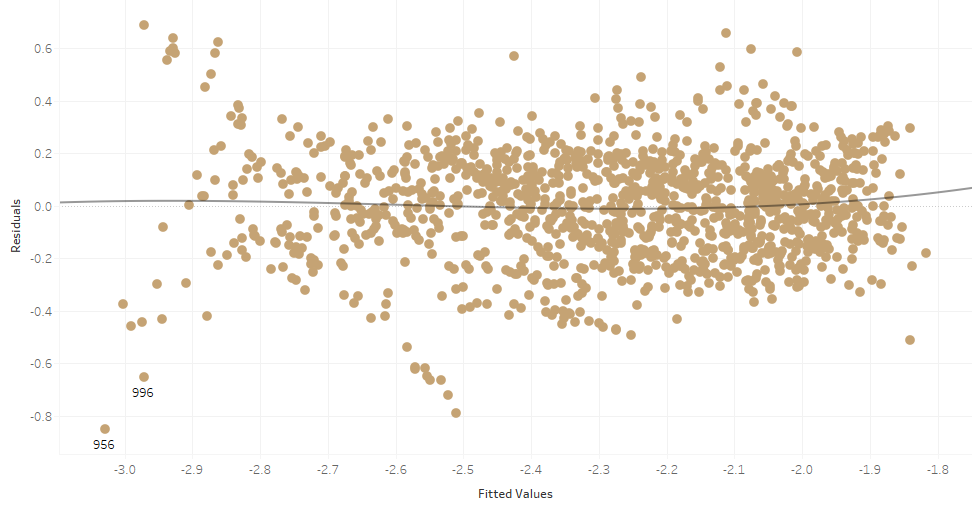
\includegraphics[width=0.8\textwidth]{Images/fitres.png}
\caption{Residuals vs Fitted plot.}
\end{center}
\end{figure}
\bigskip

Since no distinct pattern is recognizable, the relationship between the predictors and the outcome variable is assumed to be close to linear. Points 956 and 996 seem to positioned quite far from the others, on the bottom left: they are two observations from Ukraine, a country which produces electricity at a low price thanks to its natural resources. Hence, the hypothesis that those are mistaken records is discarded. \textit{Figure 2.4} shows how the residuals are distributed.

\bigskip
\begin{figure}[H]
\begin{center}
\captionsetup{justification=centering}
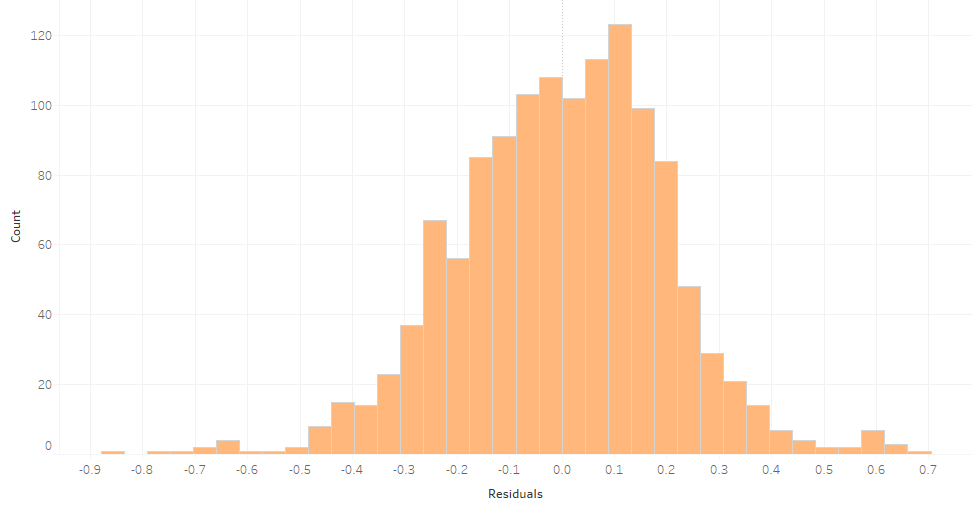
\includegraphics[width=0.8\textwidth]{Images/distres.png}
\caption{Distribution of the Residuals.}
\end{center}
\end{figure}
\bigskip

Residuals show a distribution which is slightly skewed to the left: it happens more often that the simple linear model that has been built underestimates the real value with respect to a no residual situation. However, also given the large number of data points, this small deviation from perfect normality is not too alarming. One note: to the outcome variable at hand the logarithmic transformation has been applied, so a 0.1 residual does not correspond to a 10 cents of a dollar estimation error.\\

Another problem that can pop up in regression models is the collinearity or the multi-collinearity of the predictor variables. In the presence of collinearity, the solution of the regression model becomes unstable. This hurdle can be assessed by computing a score called the variance inflation factor (or \textbf{VIF}), which measures how much the variance of a regression coefficient is inflated due to multi-collinearity in the model. \textbf{Table 2.5} displays the result of running VIF on the variables from Model 3.

\bigskip
\begin{table}[H]
\begin{center}
\begin{tabular}{|c|c|c|c|}
\hline
\rowcolor{lightgray} \multicolumn{4}{|c|}{Variance Inflation Factor}\\
\hline
&GVIF&Df&$GVIF^{\frac{1}{2*Df}}$\\
\hline
log(GAS)&2.1&1&1.4\\
DEP&2.4&1&1.5\\
log(CON)&1.4&1&1.2\\
REN&1.8&1&1.3\\
log(GDP)&2.6&1&1.6\\
log(OIL)&1.5&1&1.2\\
MAR&1.3&1&1.1\\
EU&4.9&3&1.3\\
\hline
\end{tabular}
\caption{VIF test.}
\end{center}
\end{table}
\bigskip

Since GVIF and adjusted GVIF values are rather low, well under the critical 10 threshold, multi-collinearity can be safely considered as not an issue in this case.\\

\textit{Figure 2.5} displays the scale-location plot, which is used to check homoscedasticity, i.e.\ the homogeneity of variance of the residuals. On the horizontal axis the fitted values are reported, as in \textit{Figure 2.3}, while on the vertical axis the residual value is taken in its absolute value and then transformed using a square root operation.

\bigskip
\begin{figure}[H]
\begin{center}
\captionsetup{justification=centering}
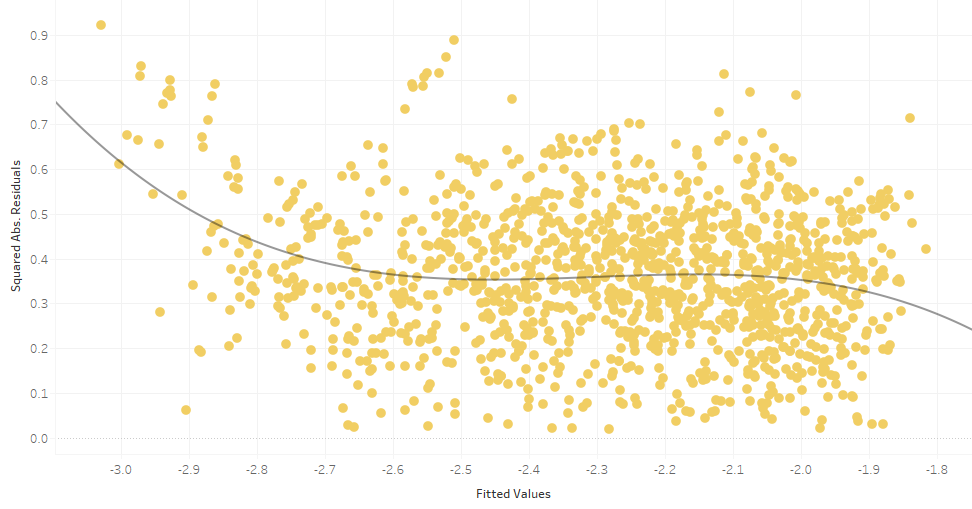
\includegraphics[width=0.8\textwidth]{Images/scalelog.png}
\caption{Scale-Location plot.}
\end{center}
\end{figure}
\bigskip

Equally spread points and consequent horizontal line of fit is a good indication of homoscedasticity: in this case, hard to give a definite answer. On the left-hand side of the plot, so when the fitted values are particularly small, the residuals tend to be greater. To investigate further, one idea is to run the \textbf{Breusch-Pagan} test, which fits a linear regression model to the previous residuals and rejects if too much of the variance is explained by the additional explanatory variables. \textit{Table 2.6} provides a summary.

\bigskip
\begin{table}[H]
\begin{center}
\begin{tabular}{|c|c|c|}
\hline
\rowcolor{lightgray} \multicolumn{3}{|c|}{BP Test}\\
\hline
BP&df&p-value\\
179&10&$<$2E-16\\
\hline
\end{tabular}
\caption{BP test.}
\end{center}
\end{table}
\bigskip

The test detects heteroscedasticity. This means that the least squares estimator is still a linear and unbiased estimator, but it may no longer be the best. That is, there is another estimator with a smaller variance. In order to correct for heteroscedasticity, a \textbf{Box Cox} transformation is applied on the dependent variable, electricity price. A transformation of this type makes a non-normal dependent variable into a normal shape. \cite{box1964analysis} Code for applying Box-Cox transformation on the dependent variable is left in the appendix: in any case, as displayed in \textit{Table 2.7}, the overall situation improves but the BP test still detects heteroscedasticity.

\bigskip
\begin{table}[H]
\begin{center}
\begin{tabular}{|c|c|c|}
\hline
\rowcolor{lightgray} \multicolumn{3}{|c|}{BP Test}\\
\hline
BP&df&p-value\\
114&10&$<$2E-16\\
\hline
\end{tabular}
\caption{BP test after having applied BC transformation on outcome variable.}
\end{center}
\end{table}
\bigskip

\subsection{Weighted Least Squares}

Another option to better deal with non-constant variance is to deviate from ordinary least squares to use weighted least squares model. Weighted least squares corrects homoscedasticity by weighting each observation by the reciprocal of its estimated variance. Observations with small estimated variances are weighted higher than observations with large estimated variances. The precise steps are reported in the appendix, but the idea is to store the residuals from \textit{Model 3} and then run a regression on the residuals themselves. The weights for the final model are then obtained by taking the reciprocal of the square root of the exponential of the fitted values from this intermediate model. Since the weights are inversely proportional to the error variance, they reflect the information in that observation. So, an observation with small error variance has a large weight since it contains relatively more information than an observation with large error variance.\textit{Table 2.8} compares the resulting coefficients from \textit{Model 3}, with Ordinary Least Squares, and the linear model with weighted regression, which is going to be referred to as \textit{Model 4}.

\bigskip
\begin{table}[H]
\begin{center}
\begin{tabular}{|c|c|c|}
\hline
\rowcolor{maroon} \multicolumn{3}{|c|}{Coefficients Comparison}\\
\hline
coef&OLS&WLS\\
\hline
intercept&-3.81&-3.71\\
log(GAS)&0.21&0.24\\
DEP&0&0\\
log(CON)&-0.1&-0.11\\
REN&0&0\\
log(GDP)&0.18&0.16\\
log(OIL)&0.32&0.3\\
MAR&0&0\\
EA&0.23&0.23\\
EFTA&0.24&0.27\\
EU&0.2&0.2\\
\hline
\end{tabular}
\caption{Comparison of Coefficients obtained through OLS and WLS.}
\end{center}
\end{table}
\bigskip

There are no major differences between the two models but the one built through Weighted Least Squares is supposed to be more robust. The interpretation of the resulting coefficients and standard errors remains the same as before.\\

It is important to note that the fact that some heteroscedasticity is detected while not using weights should not be too worrisome: most real world data is in fact heteroscedastic. If the sample size is large enough, however, the variance of the least squares estimator is supposed to be sufficiently small to get precise estimates. That is why from the following section, the use of the weights inside models is going to be carried out only sporadically.

\subsection{Subset Selection}

To have an idea of the goodness of models there are several options: one could look at the \textit{Adjusted $R^{2}$} values, as previously done in the chapter, or at some alternative accuracy metrics, as \textit{AIC}, \textit{BIC} or \textit{CP}. R squared is the proportion of variation in the outcome that is explained by the predictor variables: sadly, any variable which is added to the model is going to increase this accuracy metric, which is hence usually adjusted by the number of variables $n$. Akaike's Information Criteria (shortened AIC), Bayesian Information Criteria (shortened BIC) and Cp's basic idea is instead to penalize the inclusion of additional variables to the model. The lower the levels for these metrics, the better the model.\\

The take-home message is that having a very large model including variables which are not really significant can decrease the likelihood of the final predictions produced being reliable. The next step is to assess whether the model with all the variables from \textit{Model 3} is supposed to be the best or it is better to focus on a subset of those predictors. \textit{Table 2.9} displays the performance of the different models while one variable at a time is excluded from the model. For the steps to obtain such a table for subset selection, please refer to the appendix.

\bigskip
\begin{table}[H]
\begin{center}
\begin{tabular}{|c|c|c|c|c|}
\hline
\rowcolor{lightgray} \multicolumn{5}{|c|}{Subset Selection}\\
\hline
Excl Var&N of Vars&Adj $R^2$&BIC&Cp\\
\hline
&10&0.62&-1183&11\\
DEP&9&0.62&-1186&13\\
MAR&8&0.62&-1180&25\\
EFTA&7&0.61&-1158&52\\
EA&6&0.6&-1123&94\\
EU&5&0.59&-1092&133\\
log(CON)&4&0.57&-1058&177\\
log(OIL)&3&0.54&-966&292\\
REN&2&0.5&-858&438\\
log(GAS)&1&0.4&-647&753\\
\hline
\end{tabular}
\caption{Comparison of accuracy metrics while removing one variable at a time.}
\end{center}
\end{table}
\bigskip

The first variables to be excluded from the model are Dependence on Imports and Market Concentration, followed by the geographical dummy variables. Contrarily, log(GDP) does not appear in the table which means that it is the last variable to be left. To decide which the best model is one has to look at the accuracy metrics: adjusted $R^2$ and Cp would suggest to opt for the model including all the variables, while BIC suggests to exclude DEP.\\

The problem with the accuracy metrics described above is that they are computed on the same data set that is used for training the model. When there is enough information availability an option is to use a a part of the data to actually measure performance only. For instance, to understand which one of two models is the most reliable it is only necessary to compare the performance of the two models on the real-world data that is left for validation. In the case of the electricity data set at disposal, the idea is to split information on a temporal basis: the training set includes data prior to 2015, validation set includes the most recent information.\\

At this point, simple and weighted linear regressions are recomputed on the smaller size training set. Performance of this two models on the validation set is reported in \textit{Table 2.10}. The accuracy metric used is the \textit{Mean Absolute Error}, which is computed as the arithmetic average of the absolute errors.

\bigskip
\begin{table}[H]
\begin{center}
\begin{tabular}{|c|c|c|c|}
\hline
\rowcolor{maroon} \multicolumn{4}{|c|}{Mean Absolute Error}\\
\hline
OLS&1.81&WLS&1.89\\
\hline
\end{tabular}
\caption{Comparison of performance between OLS and WLS, measured in Euro cents.}
\end{center}
\end{table}
\bigskip

Ordinary Least Squares seems to outperform Weighted Least Squares when testing the models on the validation set. Adjusted $R^2$, BIC and Cp metrics suggested to keep all the variables in the models, or in the worst case drop DEP. Now it could be interesting to check whether also Mean Absolute Error result proves to go in this direction. \textit{Table 2.11} summarizes information regarding the best model for $N$=1,...,10 where $N$ is the number of variables in the model. Resulting Mean Absolute Error, measured in Euro cents, is reported in the final column. Models are obtained through Ordinary Least Squares.

\bigskip
\begin{table}[H]
\begin{center}
\begin{tabular}{|c|c|c|c|c|c|c|c|c|c|c|c|}
\hline
\rowcolor{lightgray} \multicolumn{12}{|c|}{Mean Absolute Error, OLS}\\
\hline
log(GAS)&DEP&log(CON)&REN&log(GDP)&log(OIL)&MAR&EA&EF&EU&NVars&MAE\\
\hline
x&x&x&x&x&x&x&x&x&x&10&1.81\\
x&&x&x&x&x&x&x&x&x&9&1.82\\
x&&&x&x&x&x&x&x&x&8&2.02\\
x&&&x&x&x&&x&x&x&7&2.05\\
x&&&x&x&x&&x&x&&6&1.97\\
x&&&x&x&x&&&x&&5&1.96\\
x&&&x&x&x&&&&&4&2.01\\
&&&x&x&x&&&&&3&2.22\\
x&&&&x&&&&&&2&2.03\\
\hline
\end{tabular}
\caption{Models obtained through OLS and corresponding error.}
\end{center}
\end{table}
\bigskip

As expected, the best performing model is the one built including all the variables of the data set. As discussed earlier, however, Ordinary Least Squares may be not the only option. It may result interesting to see what happens when the data points effect on the model is weighted through our weights $W$.

\bigskip
\begin{table}[H]
\begin{center}
\begin{tabular}{|c|c|c|c|c|c|c|c|c|c|c|c|}
\hline
\rowcolor{maroon} \multicolumn{12}{|c|}{Mean Absolute Error, WLS}\\
\hline
log(GAS)&DEP&log(CON)&REN&log(GDP)&log(OIL)&MAR&EA&EF&EU&NVars&MAE\\
\hline
x&x&x&x&x&x&x&x&x&x&10&1.89\\
x&&x&x&x&x&x&x&x&x&9&1.88\\
x&&&x&x&x&x&x&x&x&8&2.07\\
x&&&x&x&x&&x&x&x&7&2.09\\
x&&&x&x&x&x&x&&&6&2.08\\
x&&&x&x&x&x&&&&5&2.07\\
x&&&x&x&x&&&&&4&1.95\\
&&&x&x&x&&&&&3&2.23\\
&&&&x&x&&&&&2&1.75\\
\hline
\end{tabular}
\caption{Models obtained through WLS and corresponding error.}
\end{center}
\end{table}
\bigskip

Interestingly enough, the model which results as the best performing on the validation set is not the one including all the variables but the one which includes only two, Gas price and Real GDP per person. This outcome seems to oppose the idea that using all the variables is the best available option. \textit{WLS} with two variables is also able to outperform the best \textit{OLS} model by more than half a cent. All the code for measuring performance for Ordinary Least Squares, Weighted Least Squares and Exhaustive Subset Selection is left for the appendix.

\subsection{Ridge Regression}

Rather than completely excluding some predictor variables it could be beneficial to simply use smaller coefficients with respect to the ones of the linear regression model. The linear model could be wrong in assigning high coefficients to variables that are not that important, rather than being wrong in including them in the model. To shrink the coefficients one idea is to use \text{Ridge} regression: the resulting model is similar to least squares, except the coefficients are determined by minimizing a slightly different quantity, which includes a \textit{shrinkage} penalty $\lambda$. The use of the penalty has the effect of shrinking the estimates towards zero. As $\lambda$ approaches infinity, the impact of the shrinkage penalty grows, making the coefficient estimates converge to zero. \cite{james2013introduction} This property of ridge regression is showed in \textit{Figure 2.6}, in which a new model for the electricity price prediction is built.

\bigskip
\begin{figure}[H]
\begin{center}
\captionsetup{justification=centering}
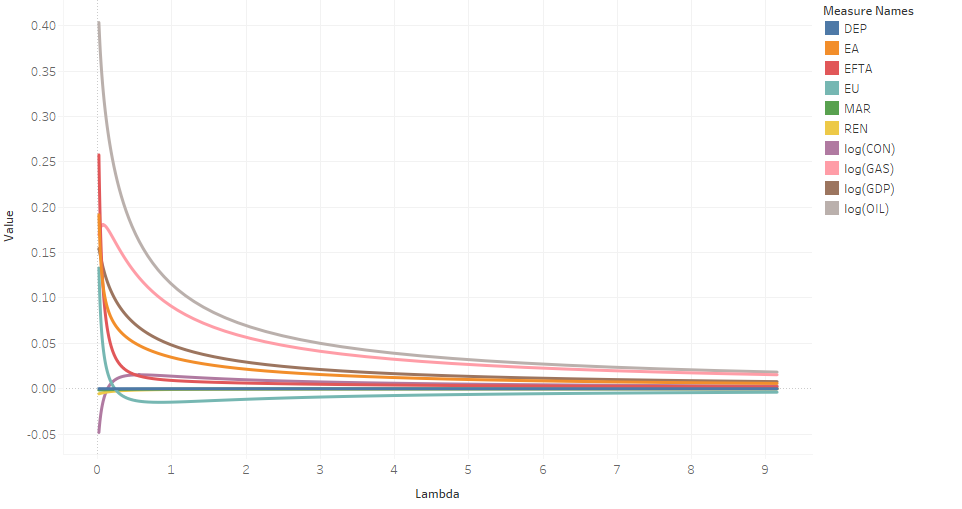
\includegraphics[width=1\textwidth]{Images/ridge.png}
\caption{Coefficient Estimates for ridge regression.}
\end{center}
\end{figure}
\bigskip

The next step is now to decide where to draw the vertical line on the graph to settle for a specific value of the parameter $\lambda$. The best way to do so is, once again, using part of the data to measure performance, in this case through cross-validation. The $\lambda$ parameter which results as the best performing is 0.018, so extremely low: this is an indication that regularizing the parameters may not be that beneficial, in this context. In fact, the average value error of the prediction with respect to the actual electricity price is of about 1.8 cents, not a real improvement with respect to previous models.

\subsection{Lasso}

One drawback of ridge regression models is that even variables that do not present any significance in the problem context do have a non-zero estimate. Ridge regression includes all predictors in the final model, since increasing the value of $\lambda$ will tend to reduce the coefficient estimates, but will result in no variable exclusion. If however the shrinkage penalty formulation is slightly changed, some of the coefficient shall be forced to be exactly equal to zero when when the tuning parameter $\lambda$ is sufficiently large. This type of regularization and it can be considered as a sort of blend between ridge regularization, because the coefficient estimates are shrunk towards zero, and subset selection, because some of the coefficient estimates are effectively turned to zero. As it was the case for ridge regression, the choice of the $\lambda$ value is critical: cross validation on the training set, once again, is going to be used to settle for a specific value of this parameter. \textit{Figure 2.7} displays how the coefficient estimates shrink to zero while the value of $\lambda$ in increased.

\bigskip
\begin{figure}[H]
\begin{center}
\captionsetup{justification=centering}
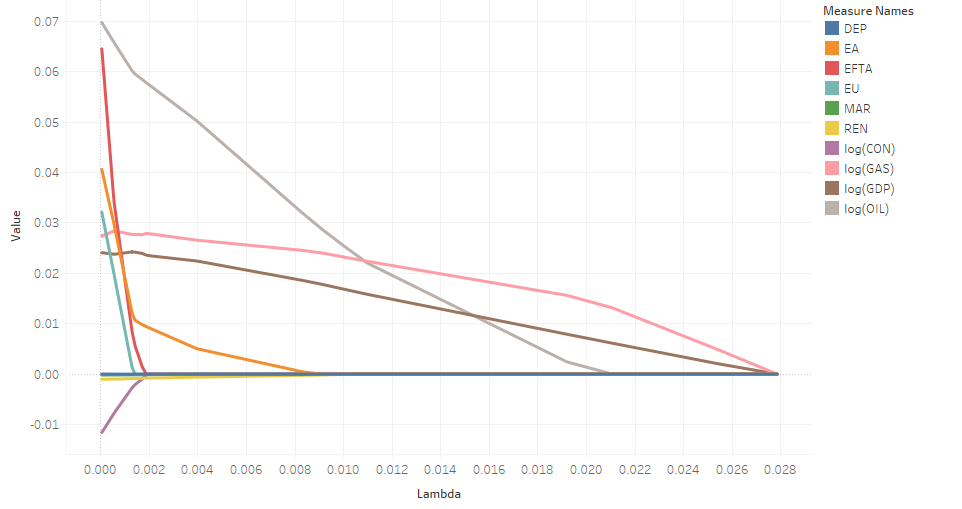
\includegraphics[width=1\textwidth]{Images/lasso.png}
\caption{Coefficient Estimates for lasso.}
\end{center}
\end{figure}
\bigskip

The way the coefficients shrink to zero is less regular with respect to what happens for ridge regression. Gas and Oil, Gdp variables are the last ones to get to zero, a further hint that they are the most significant variables at disposal. Once again, the $\lambda$ value that results as the best performing through cross validation is low, $5*10^{-5}$, so this lasso regression is quite close to linear model regression without regularization. Also the mean absolute error on the training set does not get decrease: 1.81 dollar cents. Lasso and Ridge regularization techniques respectively use so-called L1 and L2 penalties. One can go from one system to the other simply trying the model and looking at the one that performs best, but another possibility is to linearly combine the two systems, with the so-called Elastic Net regression. In this case cross validation is not only used to choose $\lambda$ but also to settle for the best $\alpha$, a parameter that allows to determine the weight of L1 with respect to the L2 penalty to be applied to the model. In this section Elastic Net is not going to be used simply because the results with these regularization techniques is rather unsatisfactory.

\subsection{Interactions and Polynomials}

For the time being one assumption was made: that the predictor variables have a linear interaction with the outcome variable. This idea is partially supported by regression plots, but some meaningful interactions may have been excluded from the model. For instance, it may be that gas price and share of renewable energy are not that significant when considered alone but the interaction, so the first multiplier by the latter, is. A situation of high gas price and simultaneous high share of renewable of energy produced may hide some meaning that only the interaction term would bring to the surface. In the case of the electricity price regression, this is exactly what happens, and the coefficient of this GAS:REN interaction term is negative, meaning that the higher its value, the lower the final electricity price. To determine which the most significant interaction terms are Subset Selection is again used, with the accuracy metric being the Mean Absolute Error on the validation set. \textit{Table 2.13} displays the coefficients and corresponding errors for the models with the lowest number of variables (which are also the best performing ones). Please note that some of the variables are still taken in their logged form.

\bigskip
\begin{table}[H]
\begin{center}
\begin{tabular}{|c|c|c|c|c|c|c|c|c|}
\hline
\rowcolor{lightgray} \multicolumn{9}{|c|}{Models with Interactions}\\
\hline
GDP&GAS:DEP&GAS:OIL&DEP:REN&CON:REN&GAS:REN&GAS:GDP&NVars&MAE\\
\hline
x&x&x&x&&&&4&2.02\\
x&&x&&x&&&3&2.1\\
&&&&&x&x&2&1.69\\
&&&&&&x&1&1.78\\
\hline
\end{tabular}
\caption{Variables and Errors of the models with interactions.}
\end{center}
\end{table}
\bigskip

Allowing the models to include interactions results in a wide use of those terms, that are often preferred to the single predictor values that were used in \textit{Model 3}. In particular, when only two variables are included as predictors, and these two variables are the interaction terms \textit{log(GAS):REN} and \textit{log(GAS):log(GDP)}, the result in performance is remarkable.\\

Looking at interaction terms is one option, but another assumption that it could be interesting to relax is that the predictor variables should enter the regression model only linearly. There may some variables, as it is the case for Dependence on Imports, which are meaningful not in their linear term, but rather in their second order polynomial. \textit{Table 2.14} illustrates which are the variables used in the models which perform best on the validation set. Only one polynomial term, DEP squared, is included, but does not seem to improve performance since the model with the lowest mean absolute error is a simple linear regression with GDP as predictor.

\bigskip
\begin{table}[H]
\begin{center}
\begin{tabular}{|c|c|c|c|c|c|c|c|}
\hline
\rowcolor{maroon} \multicolumn{8}{|c|}{Models with Polynomials}\\
\hline
GDP&OIL&REN&DEP$^2$&GAS&MAR&NVars&MAE\\
\hline
x&x&x&x&x&x&6&2.34\\
x&x&x&x&x&&5&2.22\\
x&x&x&x&&&4&2.41\\
x&x&x&&&&3&2.18\\
x&x&&&&&2&2.17\\
x&&&&&&1&1.96\\
\hline
\end{tabular}
\caption{Variables and Errors of the models with polynomials.}
\end{center}
\end{table}
\bigskip

\section{Dynamic European Models}

The results discussed in the previous section are based on static models; however, the electricity price is likely to exhibit a certain degree of path-dependency, implying that the dynamic nature of this variable should be accounted for in the model. Thus, it would be interesting to re-estimate the model in a \textbf{dynamic}-panel framework. The options at this point are two: either a lagged predictor variable, which accounts for the previous record for the same country, is created, as it is done by \cite{hyland2016restructuring}, or a different outcome variable is used, changing the scope of the regression from predicting the final price of electricity to predicting the temporal difference in price from one semester to the following. To allow for this latter idea each of the predictor variables are to be changed obtaining each observation of the data set as the difference between that variable value in that semester and the variable value in the previous semester. To put it in mathematical terms: $$ \scalebox{1.25}{$y_{t_j-t_{j-1}} = \beta_0 + \beta_1 x_{1_{t_j - t_{j-1}}} + \beta_2 x_{2_{t_j - t_{j-1}}} + ...$}$$ The process to achieve this in R is left for the appendix. In any case most of the variables and time range used are the same as for the Static models, with the exception of course that the data set is slightly shorter (it starts from the second semester of 2000 and not from the first one). The only variable from the static models which is not going to be used is OIL, because not enough data is available to have good approximations of reality in a dynamic sense. Differently with respect to the previous section, EMI is instead going to appear in all the dynamic models. The problem with using the emission intensity in the static setting is in the fact that it is does not provide any meaningful information: for instance an EMI observation equal to 101 indicates a country that is getting worse in the context of its emissions per capita. If however no information is used to characterize that country with respect to others, i.e. in this context, the absence of a country identifier, makes that information quite unuseful when used in its absolute term. In this dynamic context, instead, if the difference from one term to the next one is -1, in the case of one percent decrease in emission intensity, or 1, one percent increase in emission intensity, that information can be used to infer the direction and magnitude of the change in price.\\

Of course changing the nature of the outcome variable in this way is going to significantly decrease the Mean Absolute Error of the regression: on average, the difference from one period to the other is going to be a positive number very close to zero. So the aim shifts to creating a model that is able to predict the direction and the magnitude of the change as accurately as possible.

\bigskip
\begin{figure}[H]
\begin{center}
\captionsetup{justification=centering}
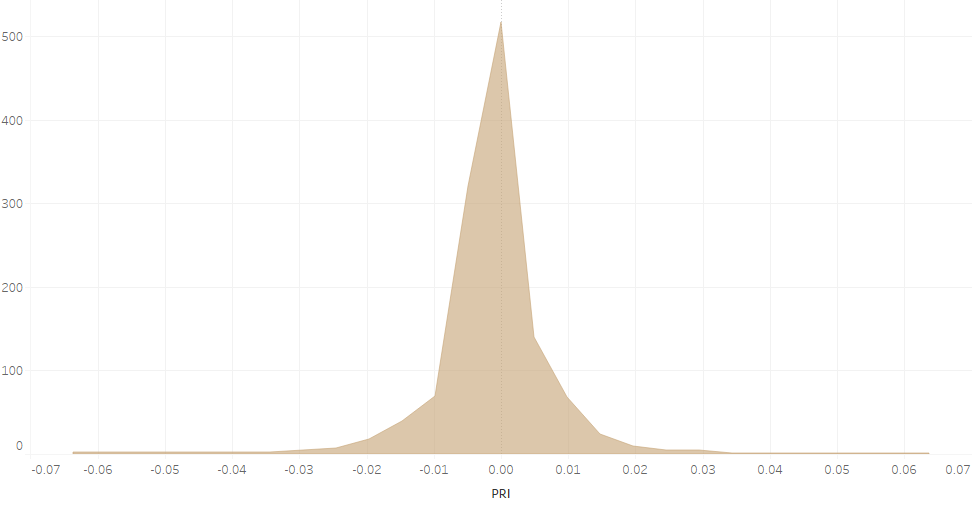
\includegraphics[width=0.8\textwidth]{Images/prihi.png}
\caption{Distribution of the outcome variable, PRI.}
\end{center}
\end{figure}
\bigskip

The first thing to be noticed is that the distribution shows long tails: most of the observations fall within a very narrow range around zero but there is also a minority number of records falling outside this span. This may later result as a problem, since normality of the outcome variable is to be assumed. In particular, one may wonder where and when the price results in a 7 cent oscillation.\\

The anomaly in the data is found in the fact that from the second semester of 2002 to the first one of 2003 the price of electricity in Norway falls by 7 cents which are then regained in the second semester of 2003. This weird behavior seems more of a recording mistake rather than a real price fluctuation experienced by the households, given that there is no hint in the data for explaining this and no sign in the literature that such an important price oscillation was effectively present. Thus, the best way out of this simply results in excluding those variables from the data set.

\subsection{Linear Model}

As it was done for the static model, the first model to be tested is linear, with multiple predictor variables. However, while in the previous section all the values showed a positive sign, in this dynamic model it will happen quite often to incur in negative observations, both for the outcome and the predictor variables. This is not a problem in the context of the linear regression, but it does not allow to apply the  simple logarithmic transformation on any of these variables. In some cases, as for the outcome PRI, some slightly more complicated transformations could be applied as for instance $log(PRI+1)$. But it would not really be worth it to go in this direction, given that there would be some significant loss in interpretability. As the linear regression name recalls, the relationship between the predictors and the outcome variable is assumed to be linear. To check whether this assumption is met, the fitted values vs residuals plot of \textit{Figure 2.9} comes in handy.\\

One note: this time the model is built directly on the training set, which is composed by observations prior to year 2015, leaving subsequent years observations to validate the results.

\bigskip
\begin{figure}[H]
\begin{center}
\captionsetup{justification=centering}
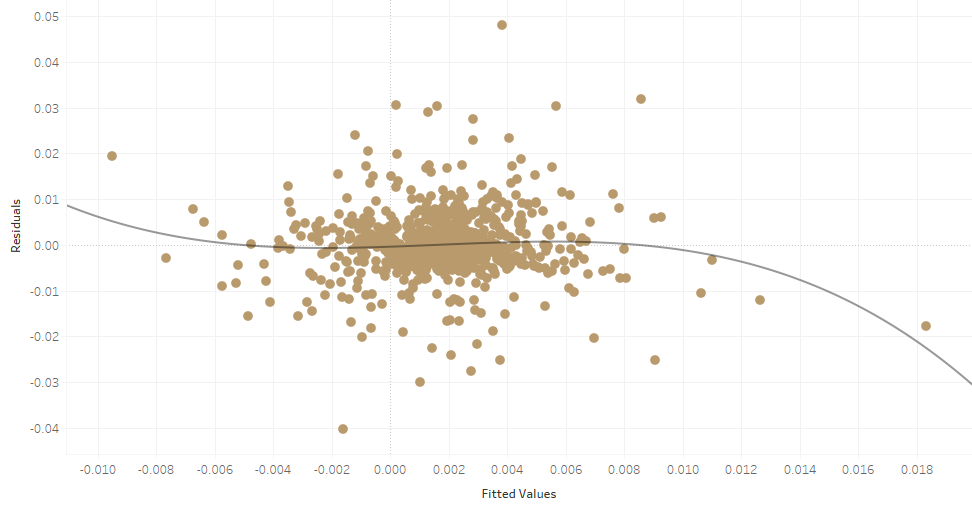
\includegraphics[width=0.8\textwidth]{Images/dynres.png}
\caption{Residuals vs Fitted plot, dynamic model.}
\end{center}
\end{figure}
\bigskip

Apart for some observations on the margins, no distinct pattern is recognizable in the most data-dense part of the plot, hinting that the relationship between the predictors and the outcome variable can be safely assumed as linear. Also, it is to be noticed how the largest residual absolute value turns out to be lower than 2 cents: keeping the 7 cents change in price would have likely messed up the regression. \textit{Figure 2.10} displays how the residuals of the regression are distributed.

\bigskip
\begin{figure}[H]
\begin{center}
\captionsetup{justification=centering}
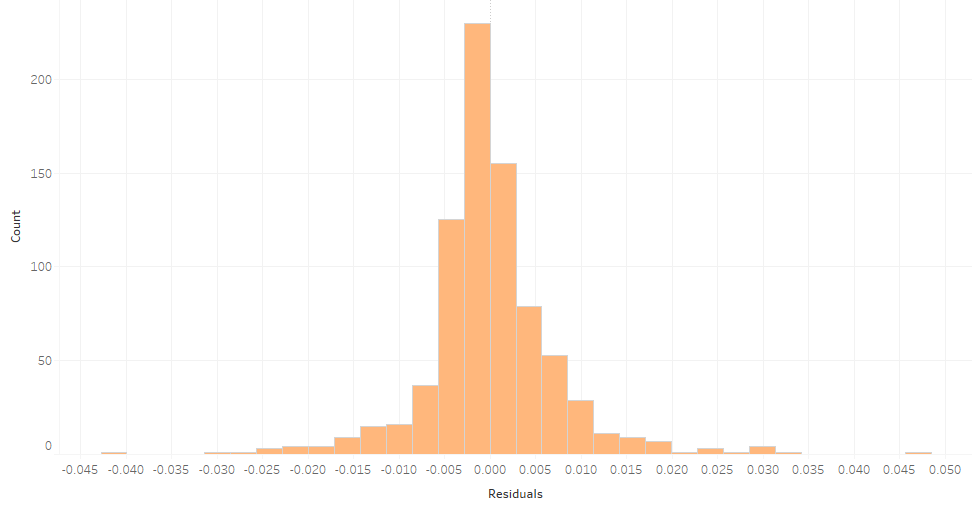
\includegraphics[width=0.8\textwidth]{Images/disres.png}
\caption{Residuals vs Fitted plot, dynamic model.}
\end{center}
\end{figure}
\bigskip

Most of the residuals fall very close to zero: 708 observations out of 800 result in less than one cent of error. The distribution shows some long tails both on the left and right side. However, given the high number of observations, this should not constitute a problem. The \textit{Variance Inflation Factor} can instead be used to check whether there is collinearity among the regression variables, as summarized by \textit{Table 2.15}. 

\bigskip
\begin{table}[H]
\begin{center}
\begin{tabular}{|c|c|c|c|}
\hline
\rowcolor{maroon} \multicolumn{4}{|c|}{Variance Inflation Factor}\\
\hline
&GVIF&Df&$GVIF^{\frac{1}{2*Df}}$\\
\hline
GAS&1.1&1&1\\
DEP&1.1&1&1.1\\
CON&1&1&1\\
EMI&1.2&1&1.1\\
MAR&1&1&1\\
REN&1.1&1&1.1\\
GDP&1.1&1&1.1\\
EU&1&2&1\\
\hline
\end{tabular}
\caption{VIF test.}
\end{center}
\end{table}
\bigskip

The GVIF and adjusted GVIF values are both very low, indicating that there is no hidden source of collinearity: the variables work independently from each other.\\

\textit{Figure 2.11} plots the Squared Root of the Absolute values of the residuals against the fitted values: the objective is to detect heteroscedasticity.

\bigskip
\begin{figure}[H]
\begin{center}
\captionsetup{justification=centering}
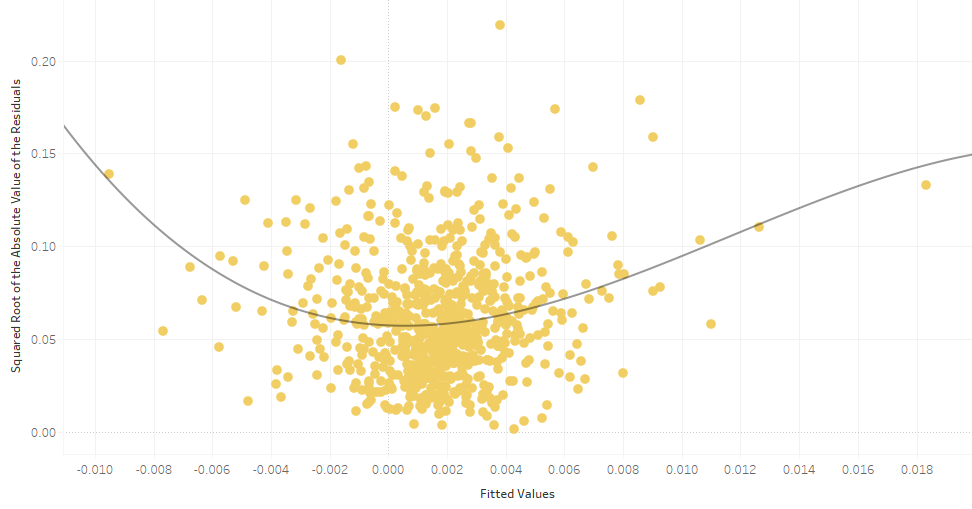
\includegraphics[width=0.8\textwidth]{Images/hetero.png}
\caption{Scale-Location plot.}
\end{center}
\end{figure}
\bigskip

When the change in price is significant, both in the positive and in the negative direction, the model is not really good in calling the right prediction. When instead the price in change is smaller, the residuals are on average small as well. This means that the model is likely to be quite conservative. Since to different values of fit correspond different residual values, the heteroscedasticity hypothesis is not to be rejected. This is an indication of the fact that the linear model with ordinary least squares may not be the best choice in the dynamic setting. \textit{Table 2.16} provides a summary of the linear regression in order to understand the impact of the predictor variables on the outcome. If the coefficient is positive, an increase in the predictor variable is going to result in an increase in the price; if instead the coefficient is negative, an increase in the predictor variable is going to result in a decrease in the price. The significance column is instead used to discriminate between variables whose coefficient is different from zero at the 95\% significance level and variables that whose coefficient those not.

\bigskip
\begin{table}[H]
\begin{center}
\begin{tabular}{|c|c|c|c|}
\hline
\rowcolor{lightgray} \multicolumn{3}{|c|}{Dynamic Linear Model}\\
\hline
&Coef Sign&Significance\\
\hline
GAS&+&***\\
DEP&+&\\
CON&-&\\
EMI&+&\\
MAR&+&\\
REN&-&\\
GDP&+&**\\
EFTA&-&\\
EU&+&\\
\hline
\multicolumn{2}{l}{\scriptsize{$^{***}p<0.001$; $^{**}p<0.01$; $^{*}p<0.05$}}
\end{tabular}
\caption{Coefficients and Significance.}
\end{center}
\end{table}
\bigskip

Differently to the static case, only two variables are significant in the dynamic setting: GDP and GAS. The change in the electricity price from one term to the other is unlikely to be explained by changes in the market concentration, use of renewables or consumption patterns. It seems that the number of variables included in the model is too large, so the focus should go on a smaller subset. However, when tested on the validation set, the models with less variables turn out performing a little bit worse with respect to the models with variables chosen through subset selection. 

\bigskip
\begin{table}[H]
\begin{center}
\begin{tabular}{|c|c|c|c|}
\hline
\rowcolor{maroon} \multicolumn{4}{|c|}{Mean Absolute Error, in Euro Cents}\\
\hline
Linear Model&0.4867&With SubSel&0.5123\\
\hline
\end{tabular}
\caption{Comparison of performance between Linear Model with and without Subset Selection.}
\end{center}
\end{table}
\bigskip

The model is wrong by less than half a cent when the model is tested on new data: this may seem as a good result, especially if compared to the accuracy of the static models. Yet, the reader should keep in mind that the outcome variable has changed with respect to the previous setting. When it is the whole electricity price to be predicted there is relatively high variability (the standard deviation of the outcome is of about 3.3 cents), while when it is only the change from one term to the other to be predicted there is low variability (the standard deviation of the outcome is of about 0.8 cents). Thus, in proportion, in the dynamic setting, a lower level of variability is captured.

\subsection{Regression Trees}

Since the linear regression models seem to not be really well-performing on this data, another option is to use regression trees. The idea behind this technique is to divide the predictor space into distinct regions $R_1, R_2, ..., R_J$. These regions have the shape of high-dimensional boxes. For each observation that falls into the region $R_j$, the same prediction, i.e. the average of the response values for the training observations in $R_j$, is output. In the case of the electricity price regression, the predictor space is created on the basis of the splits displayed of \textit{Figure 2.12}. The information used to build this tree is not the complete set: only data from years prior to 2013 are used, while the rest is left to do some parameter tuning.
 
\bigskip
\begin{figure}[H]
\begin{center}
\captionsetup{justification=centering}
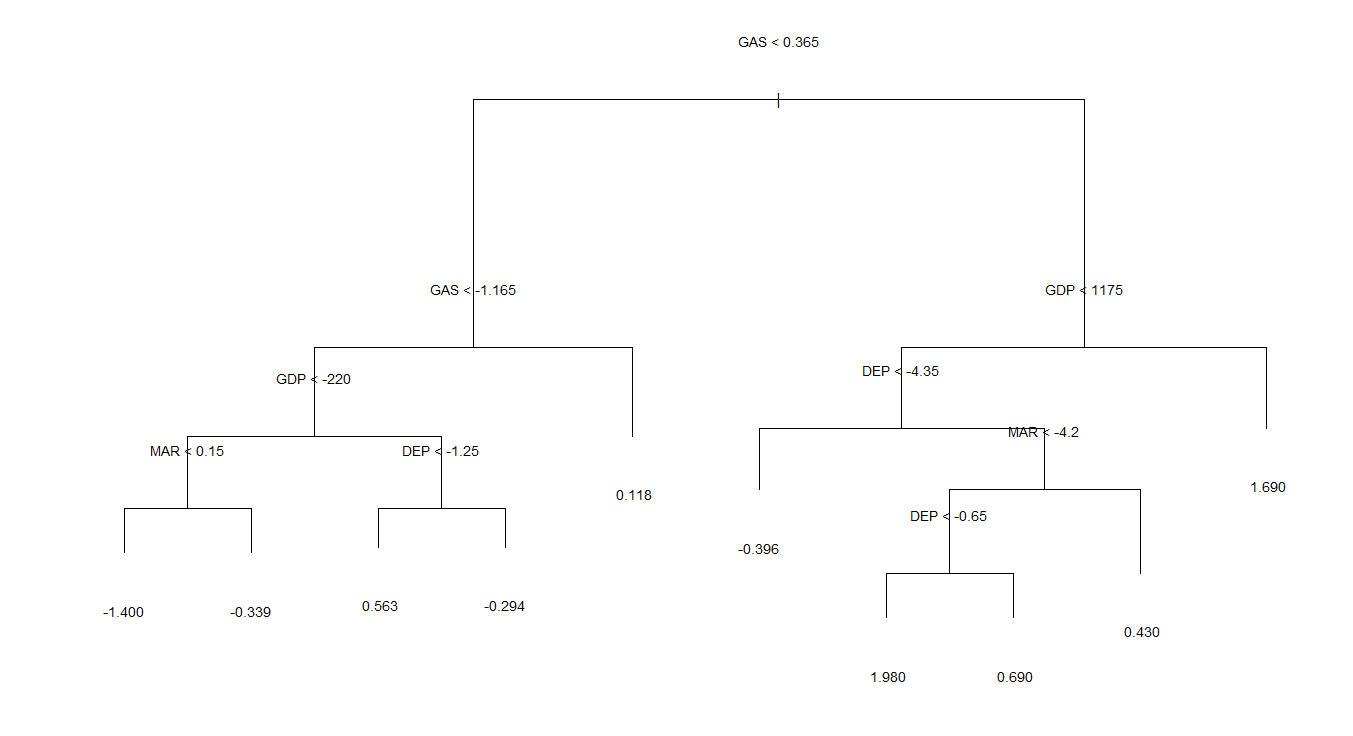
\includegraphics[width=0.8\textwidth]{Images/plot.png}
\caption{Regression Tree.}
\end{center}
\end{figure}
\bigskip

The most discriminant splits have to do with the price of natural gas: if it has gone down, then it is likely that the price of electricity will go down as well and conversely, if the former has increased, the latter will also increase. This tree excludes the possibility that, if there's been an decrease in the gas price greater than 1.2 cents, the direction of the change in electricity price is going to be positive. To further establish the magnitudes of price changes, one other predictor comes in play in particular: the real Gross Domestic Product per capita. Especially in cases of significant economy expansions (\textit{GDP} increase greater than 1175 euros), the electricity price increase is going to be particularly sizable. The two final variables that come in play are \textit{MAR} and \textit{DEP}, while there is no indication that the effect of changes in the share of renewable energy produced or in the consumption patterns do have any effect on the regression of the outcome variable.\\

The one displayed in \textit{Figure 2.12} is a complete tree, but the risk with trees is to overfit. In order to avoid this, information that was not used to build the tree (data from 2012 to second half of 2014) is employed to compute error and decide whether to reduce the number of splits in the tree or not. The total deviance of each tree in the cost-complexity pruning sequence is used as the metric to choose how many nodes to exclude. \textit{Figure 2.13} displays performance on the data left for parameter tuning. The lower the deviance, the more effective the model.

\bigskip
\begin{figure}[H]
\begin{center}
\captionsetup{justification=centering}
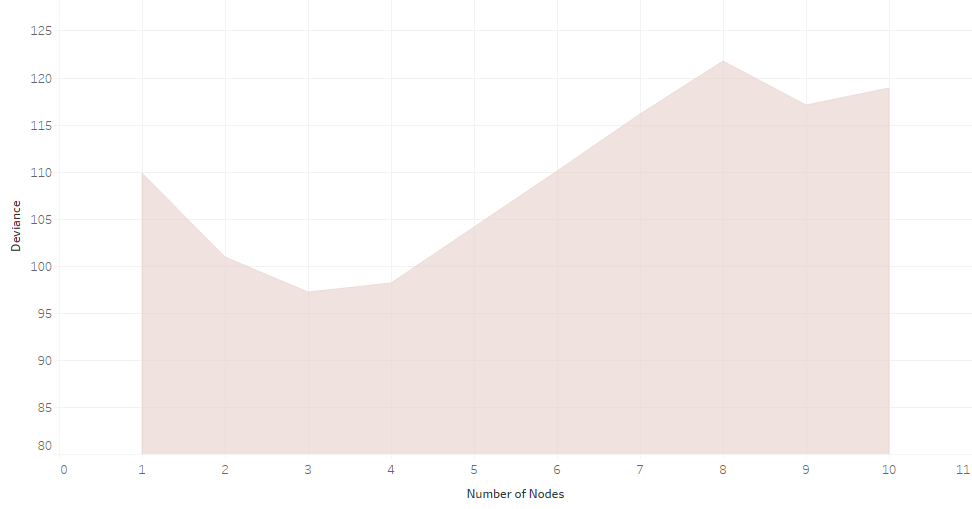
\includegraphics[width=0.8\textwidth]{Images/tre.png}
\caption{Tree Size and Relative Performance.}
\end{center}
\end{figure}
\bigskip

It seems that the complete 5-nodes model is not the best performing of the batch at all, as the deviance is lower when the number of splits is three. \textit{Figure 2.14} shows the nodes and the shape of the tree that has been pruned.

\bigskip
\begin{figure}[H]
\begin{center}
\captionsetup{justification=centering}
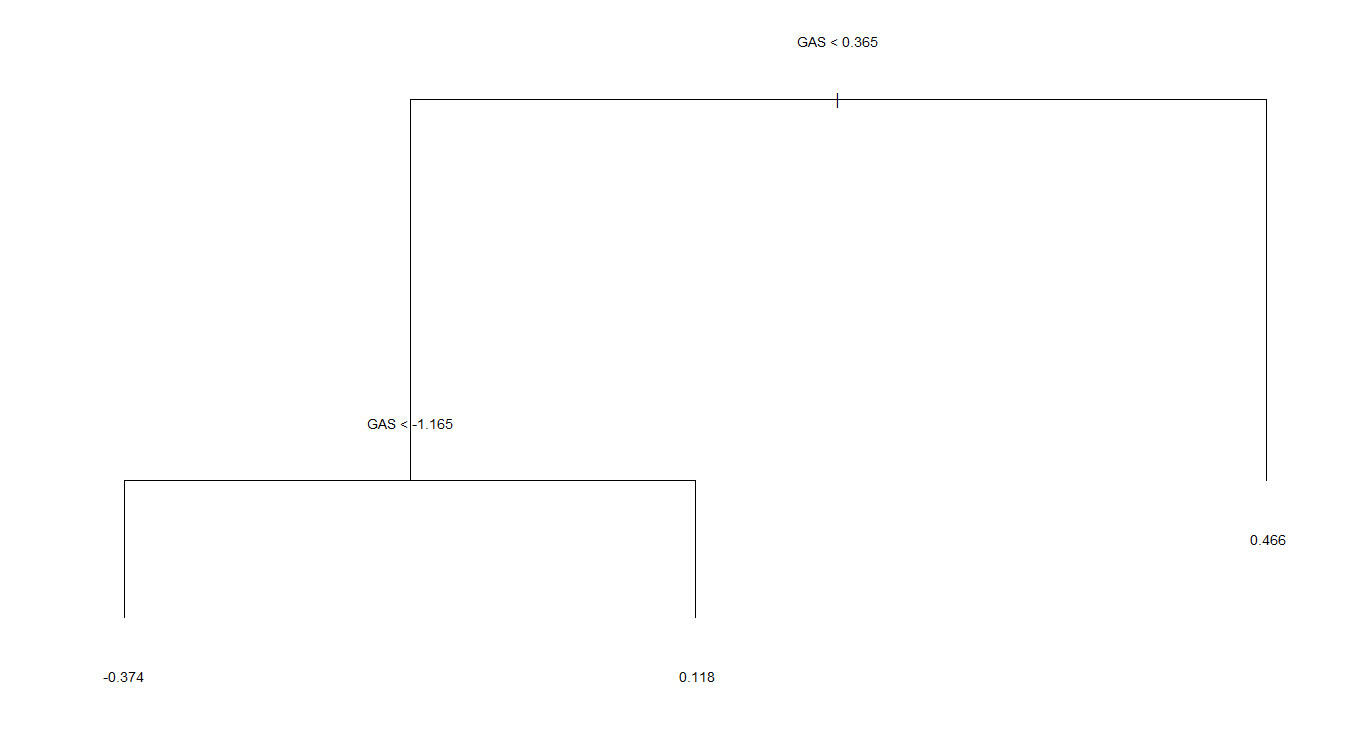
\includegraphics[width=0.8\textwidth]{Images/trep.png}
\caption{Tree after validation.}
\end{center}
\end{figure}
\bigskip

The only relevant variable that has been kept in the model is the natural gas price: when the price for this good increase, the price of electricity goes up as well. There are instead two options when the price of natural gas has decreased since the last term: if the fall has been sizable (higher than 1 cent), then the outcome value is going to be negative almost by half a cent , otherwise the electricity price increase will correspond to 0.1 cents. \textit{DEP}, \textit{MAR} and surprisingly also \textit{GDP} are excluded because their presence in the model is the result of overfitting.\\

It is now clear which the best performing tree is, but no indication yet regarding the performance on the validation set, which includes data from later years. \textit{Table 2.18} summarizes performance of the regression tree in terms of Mean Absolute Error, as previously done for the other models.

\bigskip
\begin{table}[H]
\begin{center}
\begin{tabular}{|c|c|c|c|}
\hline
\rowcolor{maroon} \multicolumn{4}{|c|}{Mean Absolute Error, in Euro Cents}\\
\hline
Tree&0.564&Pruned Tree&0.511\\
\hline
\end{tabular}
\caption{Comparison of performance between Trees before and after Pruning.}
\end{center}
\end{table}
\bigskip

The error is lower after pruning is performed with respect to the case the large model is left intact. However, overall performance does not correspond to a real step forward with respect to linear models, as it is often the case. Trees are however very simple and easy to interpret.

\subsection{Direction of Change}

The magnitude of change from one term to the other seems to be more the result of chance, rather than something that can easily be predicted. If however the problem is simplified to the prediction of only the direction of the change, the result may be more promising. The outcome variable this time is going to be the tally ``up"/``down", in relation to the change in price. The algorithm run is a generalized linear model where the outcome is binomial.\\

Also in this case it is found that the most important predictor to explain the behavior of the outcome is \textit{GAS}, while the other variables seem to not have a significant effect. The model shows performance superior to a random classifier, having the former an accuracy equivalent to 0.601 with respect to 0.5 of the latter. However, this does not come as a big improvement: the figure below on the left displays the Receiver Operative Characteristic curve for the problem at hand, while the random classifier performance (on the specificity-sensitivity basis) instead is showed on the right.

\bigskip
\begin{figure}[H]
\begin{center}
\captionsetup{justification=centering}
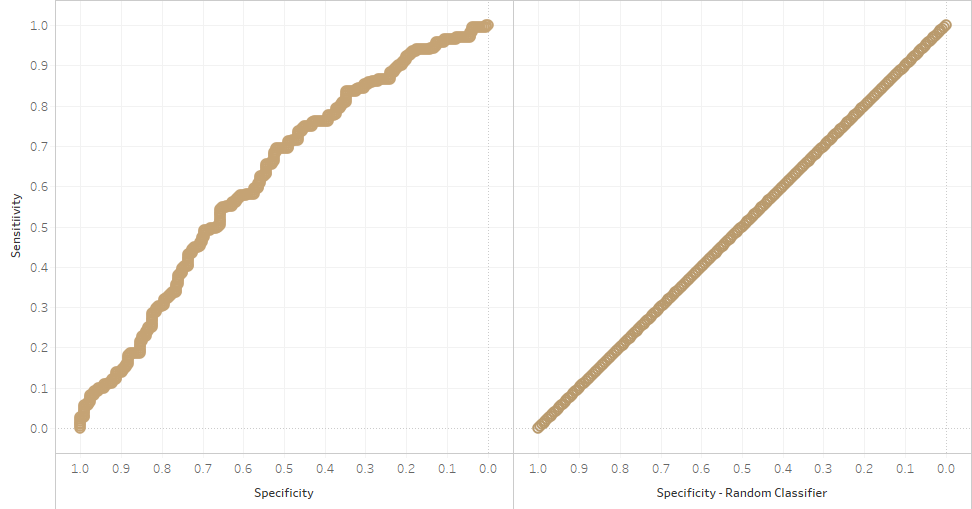
\includegraphics[width=0.8\textwidth]{Images/ROc.png}
\caption{ROC curves.}
\end{center}
\end{figure}
\bigskip

The fact that the difference between the two plots is not so striking indicates that the classifier's ability to discriminate is not strong. The take-home message from the analysis of dynamic models is that most of the variability is likely to be explained by non-systematic factors, although the natural gas price fluctuations resemble the movements in the electricity price.

\section{Global Models}

For the time being, the idea has been to focus on data from European countries, and this was the case for various reasons. The EU provides accurate and reliable information with a good frequency. Plus, for various aspects it is a common market so there are many similarities in the structure of their electricity systems. The reader may however wonder whether the findings that were discussed so far are only valid for European countries or  Excluding the rest of the world, however, may be a source of bias of the interest is in looking at global interactions between variables. The role of this section is exactly the one of providing a benchmark to European models to check whether previous findings are globally valid.

\subsection{Variables}

Data for the global analysis is taken from \textit{World Bank} instead of \textit{Eurostat}. The type of regressor variables that are used aim to resemble as much as possible the ones used for the previous regression problem. However, differences are unavoidable so variables for this new set of models have to be briefly presented.

\begin{itemize}
\item The outcome variable is, of course, the electricity price (\textbf{PRI}), which this time is measured in U.S. cents per kWh (so not in Euros as before). For the records, a monthly electricity consumption is assumed, for which a bill for the equivalent of a warehouse is computed in the largest business city for the month of March. 
\item The net of energy imports as percentage of energy use (\textbf{DEP}).
\item The Emission Intensity (\textbf{EMI}) variable is measured quite in a different way with respect to before. It is now the kg equivalent of CO2 emitted per 2010 US dollar of GDP.
\item The electric power consumption (\textbf{CON}) is measured as kWh per capita.
\item \textbf{GDP} per capita is again assessed with Purchasing Power Parity, which is a measurement of prices in different countries that uses the uses baskets of good as benchmark for the evaluating purchasing power. The principle is the same of the real GDP used by \textit{Eurostat}.
\item Pump price for gasoline, used a proxy for oil price (\textbf{OILp}), same variable as for the European discussion.
\item Electricity production from renewable sources (\textbf{REN}), excluding hydroelectric (as percentage of total).
\item Electricity production from oil sources as percentage of total, (\textbf{OILs}), is a variable which was not available from Eurostat, which only disclosed information regarding share of energy produced from renewable sources.
\item Another information data not available before that can be useful: electricity production from coal sources as percentage of total \textbf{(COA}).
\end{itemize}

The handling of information and creation of the data set is left to the appendix. One other important difference with respect to the European models is that information for the price of electricity is only available from 2015 on, so this data set is going to be wider (a very large number of countries is included) but shorter (time range only $5$ years). Since included information is also sourced from very small countries, there may be some inconsistencies: Mauritius is an island nation with a very low wealth level which is also an energy exporter (negative dependency value), but in spite of this electricity is extremely expensive, as displayed in \textit{Table 2.19}. 

\bigskip
\begin{table}[H]
\begin{center}
\begin{tabular}{|c|c|c|c|c|c|}
\hline
\rowcolor{maroon} \multicolumn{6}{|c|}{Data from Solomon Islands}\\
\hline
Year&PRI&DEP&GDP&Region&Income\\
\hline
2015&98.7&-17.4&2236&East Asia \& Pacific&Lower middle income\\
2016&99.9&-17.4&2272&East Asia \& Pacific&Lower middle income\\
2017&96&-17.4&2338&East Asia \& Pacific&Lower middle income\\
2018&67.9&-17.4&2421&East Asia \& Pacific&Lower middle income\\
2019&67.4&-17.4&2466&East Asia \& Pacific&Lower middle income\\
\hline
\end{tabular}
\caption{Data from Solomon Islands.}
\end{center}
\end{table}
\bigskip

From 2015 to 2017 one kWh was costing almost 1\$, which is an extremely high price: the effect of Mauritius observations would be very high on the model. Since the purpose of this section is to build a model that works well for most countries in the world, and it is not really of interest to accurately fit the information from a 1 million people nation, Solomon Islands observations are simply excluded from the model.

\subsection{Random Effects}

The aim is to build a model for the prediction of the electricity price that is the as global as possible, i.e. behaving well not for single countries or continents, but with observation of any provenance. From here the idea of using random effects, as if geographical information was not really of interest in this case. \textit{Table 2.20} provides a summary of the random effect model. Variables enter the model linearly, without logarithmic transformations.

\bigskip
\begin{table}[H]
\begin{center}
\begin{tabular}{|c|c|c|c|}
\hline
\rowcolor{lightgray} \multicolumn{4}{|c|}{Coefficients}\\
\hline
&Estimate&Std. Error&p\\
\hline
(Intercept)&1.39&1.49&***\\
EMI&-5.17&1&***\\
DEP&0.00&0.00&\\
CON&-0.00&0.00&\\
COA&0.07&0.01&***\\
REN&0.13&0.03&***\\
GDP&0.00&0.00&***\\
OILp&4.89&1.12&***\\
OILs&0.11&0.02&***\\
\hline
\multicolumn{2}{l}{\scriptsize{$^{***}p<0.001$; $^{**}p<0.01$; $^{*}p<0.05$}}
\end{tabular}
\end{center}
\end{table}
\begin{table}[H]
\begin{center}
\begin{tabular}{|c|c|c|c|}
\hline
\rowcolor{maroon} \multicolumn{4}{|c|}{Global Performance}\\
\hline
R-Squared&0.2431&Adj R-Squared&0.2362\\
\hline
\end{tabular}
\caption{Fixed Effects Model summary.}
\end{center}
\end{table}
\bigskip

Interestingly all three \textit{REN}, \textit{COA}, and \textit{OILs} have a positive coefficient. Although they describe opposite ways of producing energy, ranging from the most sustainable, \textit{REN}, to the most polluting, \textit{COA}, the greater the value for each variable, the greater the electricity is expected to be. Since the shares of energy produced obviously sum up to 100, this may indicate that using ways to produce electricity alternative to these (e.g. generation through gas or nuclear energy) is likely to have a negative effect on the electricity price. Or, simply, that the random effects model is not the best option for performing this type of analysis.

\subsection{Linear Model}

As the case was for the previous models, using random effects may result in a model showing little variance but too much bias. Instead, including all the country identifiers would give the opposite result. A good compromise is to use the region, which is already present in the data set and can provide some information about which parts of the world tend to have higher electricity prices with respect to others. One decision that has to be taken when building the linear model with geographical identifier is whether to use the non-percentage variables in their logarithmic form or not. If from one side a small portion of model interpretability is lost, the gain is in the reduced influence of outliers or high-leverage points. \textit{Figure 2.16} shows the difference in the residual distribution between models without (the one up) and with (the one below) logarithmic transformations. It is possible to evaluate how the second is more symmetrical, even though still a little bit skewed.

\bigskip
\begin{figure}[H]
\begin{center}
\captionsetup{justification=centering}
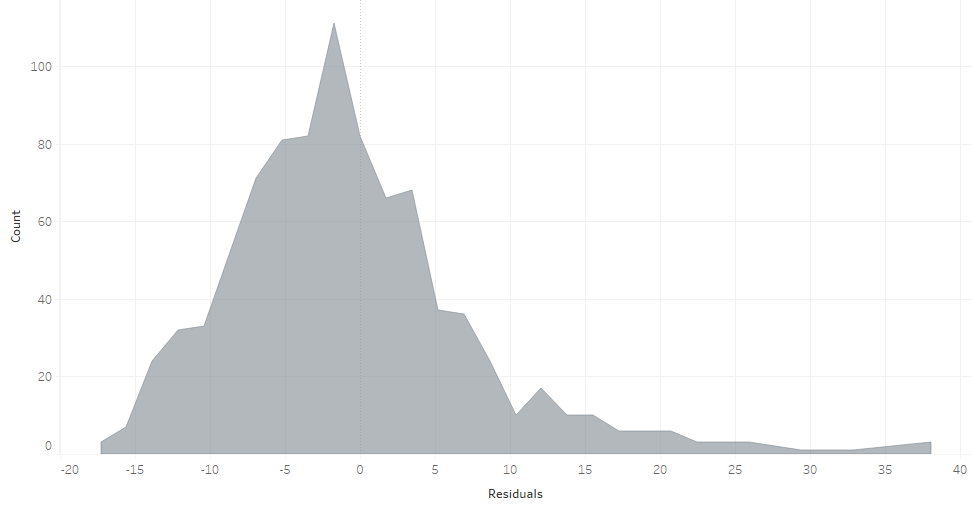
\includegraphics[width=0.8\textwidth]{Images/residualz.png}
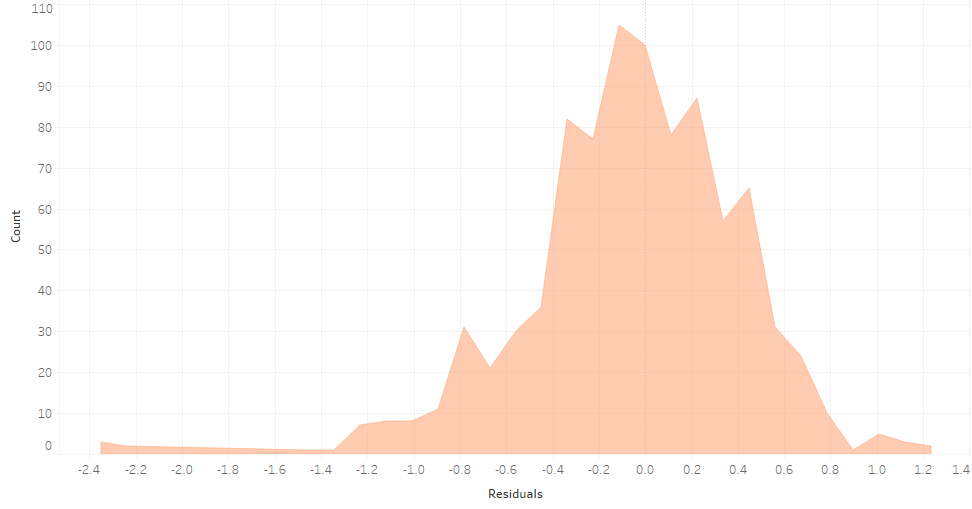
\includegraphics[width=0.8\textwidth]{Images/resdislog.png}
\caption{Residual distributions for models without and with logarithmic transformation applied on non-percentage variables.}
\end{center}
\end{figure}
\bigskip

When the logarithmic transformation is applied, also the other assumptions beside residuals' normality, as for instance homoscedasticity seem to be respected, so the model of this type is preferred. The presence of world region dummy variables allows the model to have different intercepts depending on the country in consideration. \textit{Table 2.17} displays a summary of the model with region identifier. The model is trained not on all the available observations but only on years prior to 2019, whereas last year information is left for validating the results.\\

All region dummy variables' coefficients are negative, meaning that the base case (East Asia and Pacific) is the area in which this good is the most expensive. Conversely, the price is the lowest, on average, in Middle East and North Africa (shortened \textbf{MENA}), in Europe and Central Asia (\textbf{ECA}). There is not enough information to call that the intercept for North America (\textbf{NA}) price, is significantly different from the one of the base case. For Sub-Saharan Africa (\textbf{SSA}), South Asia (\textbf{SA}) and Latin America and Caribbean (\textbf{LAC}), the intercept is lower with respect to the base case.

\bigskip
\begin{table}[H]
\begin{center}
\begin{tabular}{|c|c|c|c|}
\hline
\rowcolor{lightgray} \multicolumn{4}{|c|}{Coefficients}\\
\hline
&Estimate&Std. Error&p\\
\hline
(Intercept)&17.1&1.65&***\\
EMI&-3.7&1.04&***\\
DEP&0.01&0.00&*\\
CON&-0.00&0.00&\\
COA&0.04&0.01&**\\
REN&0.12&0.03&***\\
GDP&0.00&0.00&***\\
OILp&6.8&1.12&***\\
OILs&0.1&0.02&***\\
ECA&-9.45&0.97&***\\
LAC&-3.47&1.11&***\\
MENA&-8.02&1.26&***\\
NA&-2.94&2.75&\\
SA&-5.59&1.51&***\\
SSA&-6.5&1.07&***\\
\hline
\multicolumn{2}{l}{\scriptsize{$^{***}p<0.001$; $^{**}p<0.01$; $^{*}p<0.05$}}\\
\end{tabular}
\end{center}
\end{table}
\begin{table}[H]
\begin{center}
\begin{tabular}{|c|c|c|c|}
\hline
\rowcolor{maroon} \multicolumn{4}{|c|}{Global Performance}\\
\hline
MAE&4.959&Adj R-Squared&0.3286\\
\hline
\end{tabular}
\caption{Fixed Effects Model summary.}
\end{center}
\end{table}
\bigskip

The total variance captured by the model is about 30\%, more than with the random effects model but still quite low. However, the wide heterogeneity of the data at hand has to be considered. Interestingly, the variables \textit{OILs}, \textit{COA} and \textit{REN} still have a positive coefficient. The error on the validation set is once again measured in Mean Absolute Error (with the outcome variable re-converted with an exponential transformation) and is slightly lower than 5 dollar cents. The mean value for \textit{PRI} is 17.44 cents.

\subsection{Regularization}

The risk of leaning on linear regression is that the model fits the training data too closely, so not only the systematic component of the variance, but also unsystematic one is fit. To avoid this type of behavior, overfitting, instead of minimizing simple ordinary least squares, penalties are included in order to shrink the coefficients. In the static setting, the choice was between two alternative methods of regularization, Ridge regularization and Lasso, where the difference is in the form of the penalty term. In Ridge regression, the quantity to be minimized is: $$L_{ridge}(\hat{\beta}) = \sum\limits_{i=1}^{n}(y_i-x'_i\hat{\beta})^2 + \lambda\sum\limits_{j=1}^{m}\hat{\beta_j}^2$$, where the $\lambda$ term is the most important parameter that decides for the amount of shrinkage of the coefficients. Inside the penalty term of the Lasso regression, instead of a square operation, the absolute value of the $\beta_j$ is considered. $$L_{lasso}(\hat{\beta}) = \sum\limits_{i=1}^{n}(y_i-x'_i\hat{\beta})^2 + \lambda\sum\limits_{j=1}^{m}|\hat{\beta_j}|$$ To understand whether it is better to use ridge or lasso penalties, the best solution is to look at performance on validation set. However, it is also possible that an hybrid approach between the two results in best accuracy. This is the idea of elastic net: introducing a parameter $\alpha$ that controls for how much of each regularization to use. $$L_{elas}(\hat{\beta}) = \sum\limits_{i=1}^{n}(y_i-x'_i\hat{\beta})^2 + \lambda(\frac{1-\alpha}{2}\sum\limits_{j=1}^{m}\hat{\beta_j}^2 + \alpha\sum\limits_{j=1}^{m}|\hat{\beta_j}|)$$ The higher the $\alpha$, the closer to lasso penalization, the lower the $\alpha$, the closer to ridge regression. Best possible value has to be found not only for $\lambda$ but also for $\alpha$. To tune those parameters, cross validation is used. In the case of the electricity price regression, the value for the $\alpha$ parameter that results as best performing is 0.1, very close to straight ridge regression. \textit{Figure 2.17} displays how the coefficients shrink in the regularization process with $\alpha$ equal to 0.1.

\bigskip
\begin{figure}[H]
\begin{center}
\captionsetup{justification=centering}
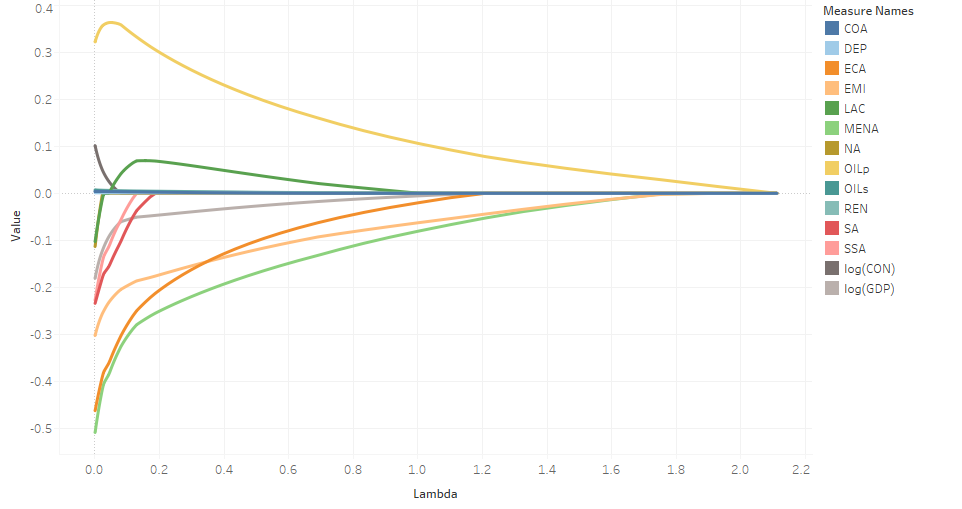
\includegraphics[width=0.8\textwidth]{Images/elastic.png}
\caption{Coefficient Estimates for the Elastic Net regression.}
\end{center}
\end{figure}
\bigskip

Despite the fact that this type of regularization is closer to $L_2$, so Ridge, than $L_1$, so Lasso, for an high enough $\lambda$ value, all coefficients shrink to zero. The corresponding $\lambda$ value, in the case of the electricity price regression is close to zero (==0.00278), and as a matter of performance there is not a great improvement with respect to the linear regression with Ordinary Least Squares (Mean Absolute Error is 4.962 cents).
\chapter{Conclusions}

\begin{appendices}
\chapter*{Data Cleaning}
The library \textit{Eurostat} is used to get the tables from the \textbf{R} interface, in particular the \textit{get\_eurostat} function. For instance, to obtain the price of electricity for years after 2007 the code is:

\begin{verbatim}
X <- get_eurostat("nrg_pc_204", time_format = "num")
X <- X[X$consom == "4161903" & X$tax == "X_TAX" & X$currency == "EUR", c(6:8)]
X <- X[!(X$geo == "EA" | X$geo == "EU27_2020" | X$geo == "EU28"),]
\end{verbatim}

To widen the data set, a series of merge functions is prompted. For instance, to add information regarding dependency from imports:

\begin{verbatim}
I <- get_eurostat("nrg_ind_id", time_format = "num")
I <- I[grep("TOTAL", I$siec), ]
I <- I[,c(3:5)]
names(I)[3] <- "DEP"
X <- merge(X, I, by=c("time", "geo"), all.x=TRUE)
\end{verbatim}

As mentioned when introducing the renewable energy share variable, the major problem is in the transition from \textit{Eurostat} to \textit{World Bank} data for information prior to 2004. In this case the library \textit{wbstats} is used, and in particular the function \textit{wb}. There are small differences in the names assigned to the countries: in \textit{Eurostat} Greece is \textbf{EL} while in the \textit{World Bank} it is \textbf{GR}, United Kingdom is \textbf{UK} while in \textit{World Bank} it is \textbf{GB}. Data integration between the two data sources is carried out using the following code:

\begin{verbatim}
J <- wb(indicator = "EG.FEC.RNEW.ZS", startdate = 2000, 
	  enddate = 2004, country=c(levels(X$geo), "GB", "GR"))
J$iso2c <- gsub("GB", "UK", J$iso2c)
J$iso2c <- gsub("GR", "EL", J$iso2c)
J <- J[,c(2,3,6)]
names(J) <- c("time", "WBren", "geo")
I <- merge(I, J, by=c("time", "geo"))
I$FAC <- I$REN / I$WBren
I <- I[,c(2,5)]
J <- merge(J, I, by="geo")
J$REN <- round(J$WBren * J$FAC, 3)
J <- J[J$time < 2004, c(1,2,5)]
U <- rbind(U, J)
X <- merge(X, U, by=c("time", "geo"), all.x=TRUE)
\end{verbatim}

For a discrete number of countries, information regarding \textit{market concentration} is sometimes missing. In the case of Bulgaria, for instance, all the values prior to 2013 are not available; those NAs are substituted with the first available year (2013).

\begin{verbatim}
X[X$geo == "BG" & X$time %in% c(2000:2012), "MAR"] 
	<- X[X$geo == "BG" & X$time == 2013, "MAR"]
\end{verbatim}

While for Bulgaria it was use possible to simply copy and paste the information from following years, the Netherlands have never disclosed any information regarding market concentration. In this case data is substituted with averages from countries with similar market structure, as Belgium, Germany, Luxembourg and Denmark.

\begin{verbatim}
for (i in 1:nrow(X)) {
  year <- X$time[i]
  if (X$geo[i] == "NL" & year%%1==0){
    DEvalue <- X[X$geo == "DE" & X$time == year, "MAR"]
    BEvalue <- X[X$geo == "BE" & X$time == year, "MAR"]
    LUvalue <- X[X$geo == "LU" & X$time == year, "MAR"]
    DKvalue <- X[X$geo == "DK" & X$time == year, "MAR"]
    NLvalue <- mean(c(DEvalue, BEvalue, LUvalue, DKvalue), na.rm=T)
    X[X$geo == "NL" & X$time == year, "MAR"] <- NLvalue
  }
}
\end{verbatim}

\textit{Eurostat}, at the time of the writing, has not yet published data regarding emission intensity for years 2019 and 2020. Since these values are likely to have changed in the last years, the assumption is that the direction of the change follows the trend of the difference from 2017 to 2018, with some inertia (equal to 0.33). The achieve this on \textbf{R}:

\begin{verbatim}
for (country in levels(X$geo)){
  if (country != "GE") {
  diff <- (X[X$time == 2018 & X$geo == country, "EMI"] -
	X[X$time == 2017 & X$geo == country, "EMI"])
  X[X$time == 2019 & X$geo == country, "EMI"] 
	<- round(X[X$time == 2018 & X$geo == country, "EMI"] + diff / 3, 1)
  X[X$time == 2020 & X$geo == country, "EMI"]
	<- round(X[X$time == 2018 & X$geo == country, "EMI"] + 2 * diff / 3, 1) }
}
\end{verbatim}

Price of natural gas tends to increase over time. For this reason, when substituting Not Availables for the Gas variable when it is missing, both the history of the price for that country and the average of countries in that year is taken into account. For countries that never disclose information regarding the natural gas price, averages from neighboring or similar countries is used. In the case of the missing value for Malta, for instance, an average of the information from Italy and Greece is used.

\begin{verbatim}
for (i in 1:nrow(X)) {
  year <- X$time[i]
  country <- X$geo[i]
  if (country \%in\% c("BE", "CZ", "DE", "EE", "EL", "LI", "LU", "MK", "PL", "PT") 
		& is.na(X[i, "GAS"])) {
      X[i, "GAS"] <- weighted.mean(c(mean(X[X$geo==country,"GAS"],na.rm=T),
		mean(X[X$time==year,"GAS"],na.rm=T)),c(0.25,0.75))
  }
  else if (country == "MT") {
    value1 <- X[X$geo == "IT" & X$time == year, "GAS"]
    value2 <- X[X$geo == "EL" & X$time == year, "GAS"]
    value <- mean(c(value1, value2), na.rm=T)
    X[i,"GAS"] <- value
  }
}
\end{verbatim}

For all other Not Availables referring to non mid-term records, for variables such as Dependence, Consumption, Inflation and Emission Intensity, both the average from the year and the average from the country is taken into consideration, using a weighted mean. This schema is implemented so that if information regarding previous years is missing, the NA can still be replaced with a reasonable value. To bring an example, the code for substituting Dependence missing values is reported below.

\begin{verbatim}
for (i in 1:nrow(X)) {
  year <- X$time[i]
  country <- X$geo[i]
  if ((is.na(X[i, "DEP"]) & year\%\%1==0)) {
      X[i, "DEP"] <- weighted.mean(c(mean(X[X$geo==country,"DEP"],na.rm=T),
	mean(X[X$time==year,"DEP"],na.rm=T)),c(0.0005,0.9995),na.rm=T)
  }
\end{verbatim}

For Gross Domestic Product missing values an additional intake of care is needed, since geographically close regions may present completely different wealth levels. In the case no historic value is found, countries that are expected to have a similar GDP are used as a benchmark. The problem with the above-mentioned technique is in the fact that using the average from historic values is likely to under-estimate the real GDP value, since for most years the economy tends to grow rather than shrink. For this reason the mean is positively adjusted by multiplying it by 1.02 (the European economy in recent years has been growing by about 2 percentage point per year on average).

\begin{verbatim}
historic1 <- c()
for (i in 1:nrow(X)) {
  year <- X$time[i]
  country <- X$geo[i]
  if (country == "XK" | country == "AL" | country == "ME" | country == "MK" | country == "BA") {
    value1 <- X[X$geo == "RO" & X$time == year, "GDP"]
    value2 <- X[X$geo == "HR" & X$time == year, "GDP"]
    value3 <- X[X$geo == "RS" & X$time == year, "GDP"]
    value4 <- X[X$geo == "BG" & X$time == year, "GDP"]
    outside <- mean(c(value1, value2, value3, value4),na.rm=T)
    value <- weighted.mean(c(outside,1.01*mean(historic1)),w=c(0.0005,0.9995),na.rm=T)
    historic1 <- c(historic1, value)
    X[i,"GDP"] <- value
  }
\end{verbatim}

The remaining missing values all refer to mid-year records. When both the following semester value and the previous semester value are present, a simple average is computed.

\begin{verbatim}
for (i in 1:nrow(X)) {
  year <- X$time[i]
  country <- X$geo[i]
  if (year \%\% 1 != 0)
    for (col in c("DEP", "CON", "EMI", "MAR", "REN", "OIL")) {
      prev <- X[X$time==(year-0.5) & X$geo==country, col]
      after <- X[X$time==(year+0.5) & X$geo==country, col]
      X[i, col] <- mean(c(prev,after),na.rm=T)
    }
}
\end{verbatim}

\section*{Membership to EU}

To understand whether the membership to the European Union corresponds to a higher electricity price, left constant all other model parameters, it is necessary to first introduce some membership dummy variables. The \textbf{EA} parameter becomes one when the country belongs to the EU Economic Area, where Euro is used as a currency; for all other member countries the identifier is simply \textbf{EU}. Among the non-member countries, the ones that agreed to join the European Free Trade Association are identified as \textbf{EFTA}.

\begin{verbatim}
for (row in 1:nrow(DP)) {
  if (as.character(DP[row, "geo"]) %in% c("BG", "RO", "CZ", "HU", "HR",
	 "SE", "DK", "PL", "UK")) {
    DP$EU[row] <- "EU"
}
  else if (as.character(DP[row, "geo"]) %in% c("NO", "IS", "LI")) {
    DP$EU[row] <- "EFTA"
  }
  else if (as.character(DP[row, "geo"]) %in% c("BE", "EL", "LT", "PT", "ES", "LU", "FR",
	 "SI", "MT", "SK", "DE", "IT", "NL", "FI", "EE", "CY", "AT", "IE", "LV")){
    DP$EU[row] <- "EA"
    }
}
\end{verbatim}

\section*{Going Dynamic}

To make the new data set dynamic the idea is to subtract from one observation the value from the same country previous semester. To do so a dictionary is built through the function \textit{hash}, a copy of the original data set is stored and then a for loop is triggered. Through this for loop, values inside the newly created data set are updated with the correct difference term by using the dictionary.

\begin{verbatim}
d <- hash()
toRemove <- c()
U <- X
X$geo <- as.character(X$geo)
for (i in 1:nrow(X)) {
  country <- X[i, "geo"]
  if (X[i, "geo"] %in% c(keys(d))) {
    U[i,c(-1,-2)] <- X[i,c(-1,-2)] - d[[country]]
  } else {toRemove <- c(toRemove, i)}
  d[[country]] <- c(X[i,c(-1,-2)])
}
X <- U[-toRemove,]
\end{verbatim}

\section*{Global Data}

Previous data were mostly obtained through \textit{Eurostat}, which however provides information only for European countries. To build a more global data set, the \textit{World Bank} is used as a provider. R library to retrieve information is \textit{WDI}. Cities and regions are removed from the data, which includes only national information.

\begin{verbatim}
W <- WDI(indicator = c("IC.ELC.PRI.KH.DB1619", "EG.IMP.CONS.ZS", "EN.ATM.CO2E.KD.GD",
"EG.USE.ELEC.KH.PC", "NY.GDP.PCAP.PP.CD", "EP.PMP.SGAS.CD", "EG.ELC.PETR.ZS",
"EG.ELC.RNWX.ZS", "EG.ELC.COAL.ZS"), start = 2014, end = 2019, extra = TRUE) 
names(W) <- c("iso2c", "country", "year", "PRI", "DEP", "EMI","CON", "GDP", "OILp",
 "OILs", "REN", "COA", "iso3c", "region", "capital", "longitude", "latitude", "income",
"lending")
W <- W[W$income != "Aggregates",]
W <- W[!is.na(W$income),]
\end{verbatim}

The novelty with this type of data retriever is that it includes information regarding the region and the income level. This can be very useful when filling Not Availables. If NA is found substitute with latest value from same country or if that is not available with the average from countries of the region in consideration. The same process is carried out to fill NAs for \textit{OIL}, \textit{REN} and \textit{COA} columns.

\begin{verbatim}
for (row in 1:nrow(W)) {
  area = W$region[row]
  if (W$year[row] == 2014 & is.na(W$DEP[row])) {
    W$DEP[row] <- mean(W[W$region == area,"DEP"],na.rm=T)
  }
}

for (row in 1:nrow(W)) {
  country = W$country[row]
  if (is.na(W$DEP[row])) {
    if (is.na(W[W$country == country & W$year == 2015,"DEP"])) {
      W$DEP[row] <- W[W$country == country & W$year == 2014,"DEP"]
    }
    else {
      W$DEP[row] <- W[W$country == country & W$year == 2015,"DEP"]
    }
  }
} 
\end{verbatim}

A similar process with respect to the one described above is carried out for filling consumption and oil NAs. The only difference is that countries with the same wealth level are used instead of countries from the same region.

\begin{verbatim}
for (row in 1:nrow(W)) {
  area = W$income[row]
  if (W$year[row] == 2014 & is.na(W$CON[row])) {
    W$CON[row] <- mean(W[W$income == area,"CON"],na.rm=T)
  }
}

for (row in 1:nrow(W)) {
  country = W$country[row]
  if (is.na(W$CON[row])) {
    if (is.na(W[W$country == country & W$year == 2015,"CON"])) {
    W$CON[row] <- W[W$country == country & W$year == 2014,"CON"]
    }
    else {
      W$CON[row] <- W[W$country == country & W$year == 2015,"CON"]
    }
  }
}
\end{verbatim}

Rows in which either \textit{PRI} or \textit{GDP} information is missing, are simply excluded from the data set.

\begin{verbatim}
W <- W[!is.na(W$PRI),]
W <- W[!is.na(W$GDP),]
\end{verbatim}

\chapter*{Models}
\section*{Static}

To create a simple linear model, the command \textit{lm} needs to be run in R. For instance, \textit{Model 3} was computed by running the following.

\begin{verbatim}
LMeP <- lm(log(PRI) ~ log(GAS) + DEP + log(CON) + REN + log(GDP) + log(OIL) + MAR + EU, DP)
\end{verbatim}

To compute analysis-of-variance tables for model objects produced by \textbf{lm}, the function \textit{anova} is used. The objective is to compare models in order to evaluate differences in significance.

\begin{verbatim}
LM <- lm(log(PRI) ~ log(GAS) + DEP + log(CON) + REN + log(GDP) + log(OIL) + MAR, DP)
anova(LM, LMeP)
\end{verbatim}

The library \textit{caret} is instead used to carry out the \textbf{Box-Cox} transformation on the outcome variable. A new model is then built upon the new outcome and the previous predictor values.

\begin{verbatim}
bpt <- caret::BoxCoxTrans(DP$PRI)
DP <- cbind(DP, nP=predict(bpt, DP$PRI))
LMeB <- lm(nP ~ log(GAS) + DEP + log(CON) + REN + log(GDP) + log(OIL) + MAR + EU, DP)
\end{verbatim}
\end{appendices}

Since applying the Box-Cox transformation to the outcome variable is not always sufficient to solve problems of non-constant variance, another option is to use \textbf{Weighted Least Regression} instead of Ordinary Least Regression. Steps are displayed below.

\begin{verbatim}
DP$resi <- LMeP$residuals
LMeR <- lm(log(resi^2) ~
 log(GAS) + DEP + log(CON) + REN + log(GDP) + log(OIL) + MAR + EU, DP)
DP$varFunc <- exp(LMeR$fitted.values)
LMwls <- lm(log(PRI) ~ log(GAS) + DEP + log(CON) + REN + log(GDP) + log(OIL) + MAR + EU,
 weights = 1/sqrt(varFunc), DP)
\end{verbatim}

To perform subset selection, the library \textit{leaps} is used. It is necessary to specify the option \textit{nvmax}, which represents the maximum number of predictors to incorporate in the model. In the case of this research \textit{nvmax} = 5, so the function will return up all the variables model, that is, it returns the best 1-variable model, the best 2-variables model, …, the best 12-variables models. Backward and forward step-wise regression is instead faster and less computationally expensive because it works as a sequential system of inclusion (or exclusion) of variables, without having to compute the best subset for each $N$ from 1 to $nvmax$. Code for performing exhaustive subset selection on R is reported below.

\begin{verbatim}
leaps::regsubsets(log(PRI) ~ log(GAS) + DEP + log(CON) + REN
+ log(GDP) + log(OIL) + MAR + EU, DP, nvmax = 12)
\end{verbatim}

To split the data set in training and validation sets on a temporal basis (before and after 2015), it is sufficient to prompt the following:

\begin{verbatim}
train <- (DP$time < 2015)
test <- (!train)
\end{verbatim}

Now the idea is to use the training set to build a model which can then be tested on the most recent validation data. To correctly determine the mean difference in US cents between the real information and the model prediction it is necessary to compute the exponential transformation on the model prediction, since in the model this variable is used in its logged form.

\begin{verbatim}
LMeP <- lm(log(PRI) ~ log(GAS) + DEP + log(CON) + REN + log(GDP) + log(OIL) + MAR + EU,
 DP, subset=train)
pred <- predict(LMeP, DP[test,])
mean(abs(DP$PRI[test] - exp(pred)))
\end{verbatim}

If instead weighted least squares was used instead of OLS for building the model:

\begin{verbatim}
DP$resi[train] <- LMeP$residuals
LMeR <- lm(log(resi^2) ~ log(GAS) + DEP + log(CON) + REN + log(GDP) + log(OIL) + MAR + EU,
 DP, subset=train)

DP$varFunc[train] <- exp(LMeR$fitted.values)
LMgls <- lm(log(PRI) ~ log(GAS) + DEP + log(CON) + REN + log(GDP) + log(OIL) + MAR + EU,
 weights = 1/sqrt(varFunc), DP, subset=train)
pred <- predict(LMgls, DP[test,])
mean(abs(DP$PRI[test] - exp(pred)))
\end{verbatim}

In the previous two models all data set variables were used, but it may be that reducing the number of variables actually boosts the performance on the validation set. To evaluate the mean absolute error between the predictions and the actual data at disposal, a vector with the errors is created in order to store the performance information. For every step N in the cycle 1-10 the best subset of variables including N of them is determined and then mean absolute error is computed. In this example the weights are used in the runs but the code is very similar if OLS is preferred to WLS.

\begin{verbatim}
W <- 1/sqrt(DP$varFunc[train])
tLM <- regsubsets(log(PRI) ~ log(GAS) + DEP + log(CON) + REN + log(GDP) + log(OIL)
+ MAR + EU, DP[train,], weights=W, nvmax = 11)
test.mat <- model.matrix(log(PRI) ~ log(GAS) + DEP + log(CON) + REN + log(GDP) + log(OIL)
+ MAR + EU, data=DP[test,])
val.errors <- rep(NA, 10)
for (i in 1:10){
  coefi <- coef(tLM, id=i)
  pred <- test.mat[,names(coefi)] \%*\% coefi
  val.errors[i] <- mean(abs(DP$PRI[test] - exp(pred)))
}
which.min(val.errors)
val.errors[which.min(val.errors)]
coef(tLM, 4)
val.errors
\end{verbatim}

The library \textit{glmnet} can be used in order to create ridge, lasso and elastic net models. In particular, the function \textit{cv.glmnet} enables to choose the parameter $\lambda$ through cross validation. A seed is set simply to make the results reproducible.

\begin{verbatim}
x <- model.matrix(log(PRI) ~ log(GAS) + DEP + log(CON) + REN + log(GDP) + log(OIL)
 + MAR + EU, DP)[,-1]
y <- DP$PRI
set.seed(35)
ridge <- cv.glmnet(x[train,], log(y[train]), alpha=0, standardize=T)
bestlam <- min(ridge$lambda)
\end{verbatim}

Now that information regarding the $\lambda$ value which enables to achieve best performance (on the training set), Mean Absolute Error is computed on the validation set.

\begin{verbatim}
ridge.pred <- predict(ridge, s=bestlam, newx=x[test,])
mean(abs(exp(ridge.pred) - y[test]))
\end{verbatim}

For the visualization of \textit{Figure 2.6} the output of the following code is used:

\begin{verbatim}
mat <- as.matrix(ridge$glmnet.fit$beta)
forplot <- data.frame(t(rbind(mat, ridge$glmnet.fit$lambda)))
\end{verbatim}

If L1 is to be used instead of L2 penalty the functions to be used do not really change: the only major difference is in the $\alpha$ value to be set inside the \textit{cv.glmnet} function. 

\begin{verbatim}
lasso.mod <- glmnet(x[train,], log(y[train]), alpha=1)
set.seed(35)
cv.out <- cv.glmnet(x[train,], sqrt(y[train]), alpha=1)
bestlam <- cv.out$lambda.min
pred <- predict(lasso.mod, s=bestlam, newx=x[test,])
C <- as.vector(coef(cv.out, bestlam))
length(C[C != 0])
mat <- as.matrix(cv.out$glmnet.fit$beta)
forplot <- data.frame(t(rbind(mat, cv.out$glmnet.fit$lambda)))
\end{verbatim}

To include interaction terms it is only necessary to create a \textit{regsubsets} object that builds models not only looking at the distinct variables but also takes in the multiplied terms.

\begin{verbatim}
tLM <- regsubsets(log(PRI) ~ (log(GAS) + DEP + log(CON) + REN + log(GDP) + log(OIL)
 + MAR)^2 + EU, DP[train,], nvmax = 30, really.big = T)
test.mat <- model.matrix(log(PRI) ~ (log(GAS) + DEP + log(CON) + REN + log(GDP) + log(OIL)
 + MAR)^2 + EU, data=DP[test,])
val.errors <- rep(NA, 30)
for (i in 1:30){
  coefi <- coef(tLM, id=i)
  pred <- test.mat[,names(coefi)] \%*\% coefi
  val.errors[i] <- mean(abs(DP$PRI[test] - exp(pred)))
}
\end{verbatim}

Until now predictor variables have only entered the linear model linearly but it may actually be that using some kind of polynomials rather than the linear term does improve performance. To build models which include polynomial terms and then compare their performance through subset selection the function \textit{regsubsets} is again used.

\begin{verbatim}
tLM <- regsubsets(log(PRI) ~ poly(log(GAS),2) + poly(DEP,2) + poly(log(CON),2)
 + poly(REN,2) + poly(log(GDP),2) + poly(log(OIL),2) + poly(MAR,2) + EU, DP[train,],
 nvmax = 18)
test.mat <- model.matrix(log(PRI) ~ poly(log(GAS),2) + poly(DEP,2) + poly(log(CON),2)
 + poly(REN,2) + poly(log(GDP),2) + poly(log(OIL),2) + poly(MAR,2) + EU, data=DP[test,])
val.errors <- rep(NA, 17)
for (i in 1:17){
  coefi <- coef(tLM, id=i)
  pred <- test.mat[,names(coefi)] \%*\% coefi
  val.errors[i] <- mean(abs(DP$PRI[test] - exp(pred)))
}
\end{verbatim}

\section*{Dynamic}

The steps for building linear models and for applying subset selection on the variables are similar to the ones already described in the past section, for the static setting. What is new is the inclusion of regression trees and logistic regression. The library \textit{tree} is used for this purpose. The training set is further divided into to smaller sets, one of which is used to tune the node quantity parameter, which controls for overfitting.

\begin{verbatim}
treeset <- C[train,]
val <- (treeset$time >= 2012)
traini <- !(val)
tre <- tree(PRI ~ GAS + DEP + CON + EMI + MAR + REN + GDP + EU, treeset, subset=traini)
plot(tre)
text(tre,cex=0.85,digits=3)
\end{verbatim}

Some information data is left to decide whether to prune the tree in order to improve performance. The function \textit{prune.tree} does the job.

\begin{verbatim}
valset <- C[val,]
my.tree <- prune.tree(tre,newdata=valset)
\end{verbatim}

To choose the final tree model among the many, the deviance is used.

\begin{verbatim}
opt.trees <- which(my.tree$dev == min(my.tree$dev))
best.leaves <- min(my.tree$size[opt.trees])
my.tree.pruned <- prune.tree(tre,best=best.leaves)
\end{verbatim}

Function \textit{glm} is used to build generalized linear models of the binomial family. If the probability computed by the model is greater than 0.5 the model is going to output a positive prediction (which in this case is going to correspond to a ``up" prediction. The confusion matrix of the classification problem can be obtained using the \textit{table} command. 

\begin{verbatim}
C$increase <- ifelse(C$PRI > 0, "Up", "Down")
C$increase <- as.factor(C$increase)
lR <- glm(increase ~ GAS + DEP + CON + GDP + REN + EMI + MAR + EU, C, family=binomial,
 subset=train)
pred <- predict(lR, C, type="response")
glm.pred=rep("Down",434)
glm.pred[pred[test] >.5]="Up"
table(prediction=glm.pred , groundtruth=C$increase[test])
mean(glm.pred == C$increase[test], na.rm=TRUE)
\end{verbatim}

The Receiver Operating Characteristic curve is used to compare performances when the 0.5 probability threshold is moved. To compute the \textit{ROC} curve the library \textit{pROC} is used.

\begin{verbatim}
C$prob <- pred
library(pROC)
ROC <- roc(increase ~ prob, C[test,])
plot(ROC)
\end{verbatim}

\bibliography{references}{}
\bibliographystyle{plain}

\end{document}